% This is a LaTeX thesis template for Monash University.
% to be used with Rmarkdown
% This template was produced by Rob Hyndman
% Version: 6 September 2016

\documentclass{monashthesis}

%%%%%%%%%%%%%%%%%%%%%%%%%%%%%%%%%%%%%%%%%%%%%%%%%%%%%%%%%%%%%%%
% Add any LaTeX packages and other preamble here if required
%%%%%%%%%%%%%%%%%%%%%%%%%%%%%%%%%%%%%%%%%%%%%%%%%%%%%%%%%%%%%%%

\author{Huize Zhang}
\title{Exploration of Judicial Facial Expression in Videos and Transcripts of Legal Proceedings}
\studentid{27478343}
\def\degreetitle{Bachelor of Commerce (Honours)}
% Add subject and keywords below
\hypersetup{
     %pdfsubject={The Subject},
     %pdfkeywords={Some Keywords},
     pdfauthor={Huize Zhang},
     pdftitle={Exploration of Judicial Facial Expression in Videos and Transcripts of Legal Proceedings},
     pdfproducer={Bookdown with LaTeX}
}


\bibliography{thesisrefs}

\begin{document}

\pagenumbering{roman}

\titlepage

{\setstretch{1.2}\sf\tighttoc\doublespacing}

\clearpage\pagenumbering{arabic}\setcounter{page}{0}

\hypertarget{acknowledgements}{%
\chapter*{Acknowledgements}\label{acknowledgements}}
\addcontentsline{toc}{chapter}{Acknowledgements}

\hypertarget{declaration}{%
\chapter*{Declaration}\label{declaration}}
\addcontentsline{toc}{chapter}{Declaration}

I hereby declare that this thesis contains no material which has been accepted for the award of any other degree or diploma in any university or equivalent institution, and that, to the best of my knowledge and belief, this thesis contains no material previously published or written by another person, except where due reference is made in the text of the thesis.

\vspace*{2cm}\par\authorname

\hypertarget{abstract}{%
\chapter*{Abstract}\label{abstract}}
\addcontentsline{toc}{chapter}{Abstract}

Decisions by courtroom Justices have been discussed broadly in the legal literature. Gender, political views and religious background of both the Justices and counsel in the case potentially influence the decisions. This paper will explore the facial behaviour of the Justices during hearings with the objective of being to assess whether it can help to predict outcomes. Audio Visual(AV) recordings and case transcripts will be computationally processed and analysed to examine the decisions of each Justice.

\clearpage\pagenumbering{arabic}\setcounter{page}{1}

\hypertarget{ch:intro}{%
\chapter{Introduction}\label{ch:intro}}

\hypertarget{background-and-motivation}{%
\section{Background and motivation}\label{background-and-motivation}}

People have attempted to predict the decisions of the Justices in the past century using judge characteristics i.e.~Gender, political views, religious background. More recently, scholars\autocites{Shullman2004illusion}{chen2018justice} have been using more information from media(i.e.~AV recording, transcript, language used by the Justices) to predict the case outcome using the U.S. Supreme Court data. On-court information has also been used to study data from High Court of Australia. \textcite{tutton2018judicial} has used an ethnographic approach to present a observational study of judicial behaviour based on watching the audio footage. Manually observing the AV recordings could lead to subjective evaluation of facial expression and this motivates us \emph{to build upon \textcite{tutton2018judicial}'s work to employ facial recognition technology to study the facial expression of the justices, which will provide a more objective result than \textcite{tutton2018judicial}}.

\hypertarget{literature-review}{%
\section{Literature review}\label{literature-review}}

The literature summary is divided into two parts: (1) current work in legal studies to understand the behaviour of the Justices and (2) existing facial recognition and emotion tagging technology.

\hypertarget{legal-study-from-a-behaviour-perspective}{%
\subsection{Legal study from a behaviour perspective}\label{legal-study-from-a-behaviour-perspective}}

There is a large law \& economics and political science literature that attempts to predict how judges will vote in court cases. Much of this focuses on the characteristics of the judge i.e.~gender, political views, religious background and characteristics of the parties in the case i.e.~gender or race of the defendant in criminal cases \autocites{Stuart1962}{Peter1984}{Combining1987}{Susan1988}{Steffensmeier2001}{Kulik2003}.

Moving from static information of the judge and parties involved, more studies start to incorporate the language used by the judge on the court to predict the decision of the Justices. \textcite{black2011emotions} has study the use of pleasant and unpleasant language by the Justices and \textcite{Shullman2004illusion} and \textcite{johnson2009inquiring} have studied the effect of frequency and content of Justices' questions. \textcite{epstein2010inferring} use a regression analysis with the number of questions asked by the Justices used to infer the winning party in a case.

More recent legal study has focused on the usage of emotion and vocal characteristics of the Justices to predict the judge's votes. Although \textcite{judicalguid} present the following code of conduct:

\begin{quote}
It is important for judges to maintain a standard of behaviour in court that is consistent with the status of judicial office and does not diminish the confidence of litigants in particular, and the public in general, in the ability, the integrity, the impartiality and the independence of the judge.
\end{quote}

and this impartiality has been highlighted in judicial demeanour by \textcite{tutton2018judicial} and \textcite{goffman1956nature}, Paul Ekman \textcite{ekman1991invited} suggests that from a behavioural perspective, some facial and vocal inflections are often unbeknown to the speakers themselves. \textcite{chen2016perceived}; \textcite{chen2017covering} and \textcite{schubert1992observing} have studied the emotion of the Justices from vocal characteristics and suggest that these vocal characteristics, especially perceived masculinity is strongly correlated with the court outcomes. \textcite{dietrich2019emotional} has used a multilevel logistic model with random effects to suggest that subconscious vocal inflections contain information that is not available from text.

Moreover, a more sizeable study by \textcite{chen2018justice} have incorporated both vocal and image information of the judge into a machine learning model to predict the judge votes and case outcome using the U.S. Supreme Court data from 1946-2014. He found that image features improved prediction of case outcomes from 64\% to 69\% and audio features improved prediction of case outcomes from 67\% to 69\%. This demonstrates the potential of incorporating facial information to understand the decision of the Justices.

The literature mentioned above is mostly conducted using the U.S. Supreme Court Database and less studies have been conducted using Australian High Court data. \textcite{tutton2018judicial} has used an ethnographic approach to study the judicial demeanour in the High Court of Australia and it is the first of its kind to use transcript and AV recordings in Australian study. The study found that Justices present a detached facial demeanour during the court in most of the time while some human display of emotions i.e.~laughter and humour have also been captured by the scholars. Tutton's work has confirmed the potential of using image information to understanding the Justices as in Chen's study, while the ethnographic approach could be biased and lead to subjective results when different people are observing the videos. Thus, building upon Tutton's study, my work fills the gap of producing objective result via utilising facial recognition technology.

\hypertarget{facial-recognition}{%
\subsection{Facial recognition}\label{facial-recognition}}

An anatomical study of the decomposition of facial muscles by \autocite{ekman1976measuring} led to the development of Facial Action Code (FAC) \autocite{ekman1978} and identification of the six universal emotions on human faces. This work has been further revised as \autocite{paulekmangroup} and has laid a solid foundation for analysing facial expression and developing facial recognition software for researchers \autocites{Kobayashi1992}{huang1997}{lien2000}{Kappoor2003}{Tong2007}{Cohn2009}{Lucey2010}.

To be able to analysis the facial expression, proper facial recognition technique is needed to first extract faces from images. Facial recognition software i.e.~DeepFace \autocite{taigman2014deepface} from Facebook and FaceNet \autocite{schroff2015facenet} from Google have also been developed for face detection. OpenFace \autocite{baltrusaitis2018openface} is the first open-sourced face recognition software that provides facial expression detection, including facial landmarking, head pose estimation, eye gaze tracking and facial action unit detection. The OpenFace toolkit has been used in different area in research including depression classification \autocites{yang2016decision}{nasir2016multimodal}, emotion study \autocites{Pan2018}{Nasir2016}{Huber2018} and even sports analytics. \autocite{kovalchik2018going}.

\hypertarget{data-collection}{%
\chapter{Data Collection}\label{data-collection}}

\hypertarget{data-processing}{%
\section{Data Processing}\label{data-processing}}

The source data for this research project is the AV recordings publicly available from the High Court of Australia \autocite{highcourtau}. Due to the requirement of resolution (more than 30px for face detection) of OpenFace, we picked up seven cases from 2018 that have less than seven judges as the sample videos for our dataset. A full list of video being processed can be found in Table \ref{tab:case-info} in the Appendix.

Multiple procedures need to be performed to obtain the numerical value of facial variables from the source videos. The entire workflow has been plotted in Figure \ref{fig:workflow}. Youtube-dl \autocite{youtube-dl} has been used to download videos from the High Court of Australia\autocite{highcourtau}. Image frames are extracted from the videos for every minute via ffmpeg \autocite{ffmpeg}, resulting in 1021 image frames (252 frames from \texttt{Nauru} videos and 769 frames from other five videos). Taipan \autocite{Taipan} is then used to find the x-y coordinates of the location of the Justices in each image frame. ImageMagick \autocite{ImageMagick} is followed to crop the face of each Justice from each image frame that is taken from each video where three Justices present in \texttt{Nauru} videos and five Justices in other videos. The resulting 4601 cropped images are then sent to OpenFace \autocite{baltrusaitis2018openface} to produce the variables for facial landmarking, head pose, eye gaze and facial action unit. This step is performed via the docker platform. The resulting outputs from OpenFace are individual comma-separated values (csv) files for each of the 4601 faces considered and processing is done in R to combine all the separate csv files into a final dataframe with appropriate index of \texttt{frame}, \texttt{judg} and \texttt{video}.

\begin{figure}

{\centering 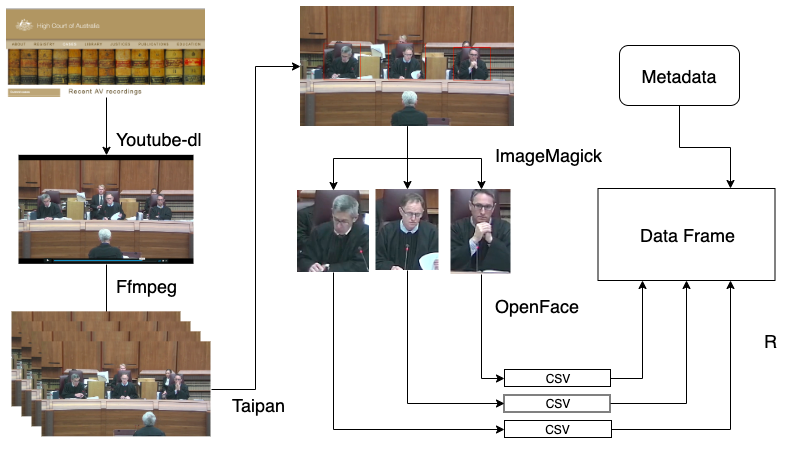
\includegraphics[width=1\linewidth]{figures/workflow} 

}

\caption{workflow for video and image processing \label{fig:workflow}}\label{fig:unnamed-chunk-1}
\end{figure}

\hypertarget{variable-description}{%
\section{Variable description}\label{variable-description}}

OpenFace provides more than 711 variables measuring different aspects of a given face and a full description of the output variables can be found in \textcite{baltrusaitis2018openface}. This outlines the difficulty of this project: no existing models will present accurate prediction and inference using 700+ variables - how can we incorporate these information to say about the facial expressions of the Justices during the hearings?

I conduct some exploratory data analysis on one video: \texttt{Nauru\_a} and find the 700+ variables can be classified as follows with some insights

\begin{itemize}
\item
  \textbf{Confidence}: How confidence OpenFace is with the detection. Confidence is related to the angle that the Justice's face present in the images.
\item
  \textbf{Gaze}: Gaze tracking: the vector from the pupil to corneal reflection. The dataset contains information on the gaze for both eyes while there is no distinct difference between the eyes. Also I was trying to make animation to track the change of the gaze for judges but no good luck.
\item
  \textbf{Pose}: the location of the head with respect to camera. Pose-related variables don't provide much useful information apart from gaze-related variables.
\item
  \textbf{Landmarking}: landmarking variables for face and eyes. Landmarking variables allows me to plot the face of the judge in a particular frame. More work could be done to explore the usefulness of landmarking variables.
\item
  \textbf{Action Unit}: Action units are used to describe facial expressions. The action unit has intensity measures ending with \texttt{\_c} and presence measures ending with \texttt{\_r}.
\end{itemize}

\hypertarget{data-format}{%
\section{Data format}\label{data-format}}

In this project, we will make use of the action unit variables along with all the added indexes to analyse the face of the judge. In the wide format, apart from the first four index columns, each action unit has two columns with one for binary presence value and another for numeric intensity value. The Table \ref{tab:wide} presents the first five rows of the dataset with columns for the first action unit only.

\begin{table}[ht]
\begin{center}
\caption{\label{tab:wide} data in wide format}
\begin{tabular}{lllllllllllllllllllllllllllllllllllllll}
\toprule
judge & video & frame & AU01-r & AU02-r & AU04-r & AU05-r & AU06-r & AU07-r & AU09-r & AU10-r & AU12-r & AU14-r & AU15-r & AU17-r & AU20-r & AU23-r & AU25-r & AU26-r & AU45-r & speaker & AU01-c & AU02-c & AU04-c & AU05-c & AU06-c & AU07-c & AU09-c & AU10-c & AU12-c & AU14-c & AU15-c & AU17-c & AU20-c & AU23-c & AU25-c & AU26-c & AU28-c & AU45-c \\
\midrule
Bell & McKell & 1 & 0 & 0 & 0.69 & 0.63 & 0 & 1.5 & 0 & 0 & 0 & 0 & 0 & 0 & 0.05 & 0 & 0 & 0.26 & 0.47 & Appellent & 0 & 1 & 1 & 0 & 0 & 1 & 1 & 0 & 0 & 0 & 1 & 0 & 1 & 0 & 1 & 0 & 0 & 0 \\
Bell & McKell & 2 & 0 & 0 & 0.69 & 0.63 & 0 & 1.5 & 0 & 0 & 0 & 0 & 0 & 0 & 0.05 & 0 & 0 & 0.26 & 0.47 & Appellent & 1 & 1 & 1 & 1 & 1 & 1 & 1 & 0 & 0 & 1 & 1 & 0 & 1 & 0 & 0 & 0 & 0 & 0 \\
\bottomrule
\end{tabular}
\end{center}
\end{table}

The data can also be expressed in the long format with action unit being another index and presence and intensity being two columns. The Table \ref{tab:long} presents the first five rows of the data in the long format.

\begin{table}[ht]
\begin{center}
\caption{\label{tab:long} data in long format}
\begin{tabular}{lllllll}
\toprule
judge & video & frame & speaker & AU & presence & intensity \\
\midrule
Edelman & McKell & 1 & Appellent & AU01 &  0 & 0.05 \\
Edelman & McKell & 1 & Appellent & AU02 &  1 & 0.00 \\
Edelman & McKell & 1 & Appellent & AU04 &  0 & 0.01 \\
Edelman & McKell & 1 & Appellent & AU05 &  0 & 0.00 \\
Edelman & McKell & 1 & Appellent & AU06 &  0 & 0.00 \\
Edelman & McKell & 1 & Appellent & AU07 &  0 & 0.00 \\
Edelman & McKell & 1 & Appellent & AU09 &  0 & 0.26 \\
Edelman & McKell & 1 & Appellent & AU10 &  0 & 0.00 \\
Edelman & McKell & 1 & Appellent & AU12 &  0 & 0.00 \\
Edelman & McKell & 1 & Appellent & AU14 &  1 & 1.23 \\
Edelman & McKell & 1 & Appellent & AU15 &  0 & 0.46 \\
Edelman & McKell & 1 & Appellent & AU17 &  0 & 0.66 \\
Edelman & McKell & 1 & Appellent & AU20 &  1 & 1.44 \\
Edelman & McKell & 1 & Appellent & AU23 &  0 & 0.64 \\
Edelman & McKell & 1 & Appellent & AU25 &  0 & 0.00 \\
Edelman & McKell & 1 & Appellent & AU26 &  0 & 0.00 \\
Edelman & McKell & 1 & Appellent & AU28 & NA &   NA \\
Edelman & McKell & 1 & Appellent & AU45 &  0 & 0.25 \\
Edelman & McKell & 2 & Appellent & AU01 &  1 & 0.05 \\
Edelman & McKell & 2 & Appellent & AU02 &  1 & 0.00 \\
Edelman & McKell & 2 & Appellent & AU04 &  1 & 0.01 \\
Edelman & McKell & 2 & Appellent & AU05 &  0 & 0.00 \\
Edelman & McKell & 2 & Appellent & AU06 &  0 & 0.00 \\
Edelman & McKell & 2 & Appellent & AU07 &  0 & 0.00 \\
Edelman & McKell & 2 & Appellent & AU09 &  0 & 0.26 \\
Edelman & McKell & 2 & Appellent & AU10 &  0 & 0.00 \\
Edelman & McKell & 2 & Appellent & AU12 &  0 & 0.00 \\
Edelman & McKell & 2 & Appellent & AU14 &  1 & 1.23 \\
Edelman & McKell & 2 & Appellent & AU15 &  1 & 0.46 \\
Edelman & McKell & 2 & Appellent & AU17 &  1 & 0.66 \\
Edelman & McKell & 2 & Appellent & AU20 &  1 & 1.44 \\
Edelman & McKell & 2 & Appellent & AU23 &  0 & 0.64 \\
Edelman & McKell & 2 & Appellent & AU25 &  0 & 0.00 \\
Edelman & McKell & 2 & Appellent & AU26 &  0 & 0.00 \\
Edelman & McKell & 2 & Appellent & AU28 & NA &   NA \\
Edelman & McKell & 2 & Appellent & AU45 &  0 & 0.25 \\
\bottomrule
\end{tabular}
\end{center}
\end{table}

\hypertarget{missing-value-imputation}{%
\section{Missing value imputation}\label{missing-value-imputation}}

The missingness in the dataset could be due to the fact that a judge is reading the materials on the desk so the face is not captured for a particular frame or simply because some faces are not detectable for the given resolution of the video stream. However, since that data is in time series structure, simply drop the missing observation will cause the time interval to be irregular and complicate further analysis.

There are two different sets of variables that need imputation. \texttt{Presence} is a binary variable that takes value of one if an action unit is present in a particular frame for a judge in a video and \texttt{Intensity} measures how strong that action unit is. Linear interpolation from \texttt{forecast} package is suitable to impute \texttt{Intensity} and \texttt{Presence} is imputed through sampling from binomial distribution. The imputed action unit data is stored as \texttt{au\_imputed} under the \texttt{raw\_data} folder.

\hypertarget{data-cleaning}{%
\section{Data cleaning}\label{data-cleaning}}

There is a data quality issue coming from the data I get from OpenFace. For some observations, the intensity of the action unit could be high while the present variable has a zero value. This does not make sense since if an action unit has been detected as strong intensity for a judge in a particular frame, it should at least present on the judge's face. Therefore, I adjust for the presence value if the intensity is higher than one. One is being chosen as the threshold value since in Ekman's definition of the intensity of the action unit, a score of one means the action unit is at least slightly present in the judge's face. The adjusted data is stored as \texttt{au\_tidy} under the \texttt{raw\_data} folder.

\hypertarget{method}{%
\chapter{Method}\label{method}}

\hypertarget{notation}{%
\section{Notation}\label{notation}}

Let \(\mathbf{X}\) be a matrix of predictors, and \(\mathbf{Y}\) variable in our case is bivariate matrix of response variables, including a binary indicator of presence/absence and a numeric value measuring intensity, of facial action unit, where

\begin{itemize}
\item
  \(X_1\) indicates \texttt{judge} with six categories \(i = 1,2, \cdots, 6\)
\item
  \(X_2\) indicates \texttt{video} for each of the seven cases, \(j = 1,2, \cdots, 7\)
\item
  \(X_3\) indicates action unit containing 18 possible facial expression.
\item
  \(X_4\) indicates \texttt{speaker}, either the appellant or respondent, \(l=1,2\)
\item
  \(X_5\) indicates \texttt{frame} corresponding to time, \(t = 1,2, \cdots, T_j\)
\end{itemize}

Note that \(t\) could be considered a time variable, but because images are taken at 1 minute intervals, temporal dependence is unlikely to exist. Rather this should be considered an independent observation.

A full, main effects model for the data might be expressed as:

\[Y_{ijklt} = \mu + \alpha_i + \beta_j + \gamma_k + \delta_l + \varepsilon_{ijklt}\]

\noindent Also, let \(P_{jitkl}\) represent the response variable presence, and \(I_{jitkl}\) represent the response variable intensity. This notation will be helpful for defining the plots and models explained in this section.

\hypertarget{modelling}{%
\section{Modelling}\label{modelling}}

\hypertarget{model-1-action-unit}{%
\subsection{Model 1: Action unit}\label{model-1-action-unit}}

A binomial model with logistic link is first used to model the presence score. Interaction of judge and action unit is included to capture the judge-wise differences for different action units. The is necessary since from the exploratory data analysis, different judges have different average presence score for different action units. The model can be written down as Equation \ref{eq:judge_au}.

\begin{equation}\label{eq:judge_au}
P_{ik} = \mu + \alpha_i + \gamma_k + (\alpha\gamma)_{ik}
\end{equation}

\hypertarget{model-2-video}{%
\subsection{Model 2: Video}\label{model-2-video}}

Build upon the first model, the second model adds the video related main effect and interactions, as shown in Equation \ref{eq:judge_video}. The interactions allow both judge and action unit variables to differ in different videos, which is useful to answer the research questions \emph{whether the judges are behaving same or different across videos}.

\begin{equation}\label{eq:judge_video}
P_{ijk} = \mu + \alpha_i + \beta_j +\gamma_k + (\alpha\beta)_{ij} + (\alpha\gamma)_{ik} + (\beta\gamma)_{jk}
\end{equation}

\noindent 

\hypertarget{model-3-speaker}{%
\subsection{Model 3: Speaker}\label{model-3-speaker}}

Build upon the second model, the third model is aimed to capture the speaker-wise effect, that is, \emph{do the expressions of the judges change when different parties are speaking}. The model formula is shown in Equation \ref{eq:judge_speaker}.

\begin{equation}\label{eq:judge_speaker}
P_{ijkl} = \mu + \alpha_i + \beta_j +\gamma_k + \delta_l + (\alpha\beta)_{ij} + (\alpha\gamma)_{ik} + (\beta\gamma)_{jk} + (\alpha\delta)_{il}
\end{equation}

Interactions are still included in this model, but attention need to be paid to ensure the interactions are relevant. Theoretically, we could include speaker with all of the three existing variables (judge, action unit and video), but this would cause the model to run out of degree of freedom given the number of observations we have. Therefore, we only include judge-speaker interaction because it is directly related to the research question of this model.

\hypertarget{diagnostics}{%
\subsection{Diagnostics}\label{diagnostics}}

The analysis of variance (ANOVA) is a statistical method that compares the mean of each treatment level for a variable. Three types of ANOVA test are designed for different purposes. Type I takes a sequential approach to test the significance of variables, thus the order of the variable in the model will potentially affect the ANOVA result. Type II ANOVA tests the main effect of a covariate after controlling for other covariates but not interactions. This approach is recommended if the interactions are not significant. Type III ANOVA tests the main effect of a covariate after controlling for other covariates \emph{and} the interactions. It is better than Type II ANOVA if the interactions are significant.

Different packages in R conduct ANOVA test: \texttt{anova()} and \texttt{drop()} from base R provides type I and type II tests. \texttt{Anova()} from \texttt{car} package allows for both type II and III through specifying a \texttt{type} argument. \texttt{aov()} from \texttt{stats} package allows for ANOVA test only for balanced dataset.

The ANOVA test provide variable significance, which allows us to understand if at least one treatment in the group is significantly different from others. This is useful before proceeds to the multiple comparison procedure, where we are able to talk which treatment(s) are different from others.

\hypertarget{post-model-analysis}{%
\section{Post-Model Analysis}\label{post-model-analysis}}

The estimates of variables from the model summary are not particularly useful in our case. This is because firstly, the estimates of the coefficient are not interpretable in the logistic regression. Secondly, we are interested in whether the mean for each treatment is same or different. Thus estimated marginal mean and multiple comparison is necessary to compute for post-model analysis.

\hypertarget{estimated-marginal-mean-emm}{%
\subsection{Estimated Marginal Mean (EMM)}\label{estimated-marginal-mean-emm}}

The estimated marginal mean is the fitted value from a model over a pre-defined reference grid. In our data, the unique combination of judge, video and action unit forms the reference grid. The estimated marginal mean is computed on each grid point as a linear fit of the model, along with standard error and confidence interval. The probability from estimated marginal mean have a nice interpretation as the estimated probability of presence score for a particular combination of action unit, judge and video. This output allows us to compare how the estimated presence probabilities of each judge, video and action unit combination are different or similar from each other.

\hypertarget{multiple-comparisons}{%
\subsection{Multiple Comparisons}\label{multiple-comparisons}}

Multiple comparison procedures consider the problem of simultaneous inference. A 5\% significance level indicates if we conduct 100 tests simultaneously, about 5 tests will show significance out of randomness. This is a problem we need to pay attention to when comparing the estimated presence probability or we may wrongly conclude judges has a different facial expression than others but they are actually not.

When multiple estimated mean are compared at the same time, the confidence level (or \(\alpha\) in p-value) need to be adjusted to control the family-wise error rate to be less than \(\alpha\). Bonferroni adjustment makes the adjustment to reject a hypothesis test at \(\alpha/N\) level so that the type I error of whole family of the simultaneous tests (Family-wise Error Rate (FWER)) is control be less than \(\alpha\). This can be proved using Boole's inequality if we denote the number of true \(H_0\) as \(N_0\).

\[\Pr\left[\bigcup \Pr(P_i \le\frac{\alpha}{N})\right] \le \sum \Pr\left(p_i \le \frac{\alpha}{N}\right) = N_0\frac{\alpha}{N} \le \alpha\]

Testing significance based on p-value has been long criticised for its interpretation. Researchers can erroneously conclude significance because of p-value being less than 0.05 without discussing the false positive/negative proportion. On the other hand, confidence interval provides a confidence range for the estimates to highlight the uncertainty around estimation. Thus I will compute the confidence interval to compare whether the estimated mean for a particular judge-AU group is same or different across videos based on if the intervals overlap with each other.

\hypertarget{results}{%
\chapter{Results}\label{results}}

\hypertarget{model-1-action-unit-1}{%
\section{Model 1: Action unit}\label{model-1-action-unit-1}}

\hypertarget{mean-presence-score-and-most-common-action-units}{%
\subsection{Mean presence score and most common action units}\label{mean-presence-score-and-most-common-action-units}}

The average presence (\(P_{ik}\)) of each action unit is first computed for each judge as \[P_{ik} = \frac{\sum_{jt}X_{ijtk}}{\sum_{j = 1}^JT_j}\] This is then plotted in Figure \ref{fig:mean_presence} to give an overview of the presence score of all the action units across all the judges. The order of action unit on the y axis is ranked by the average presence of all the judges. The five most frequent action units are highlighted in blue for each judge and summarised in Table \ref{tab:most_common}

\begin{figure}

{\centering 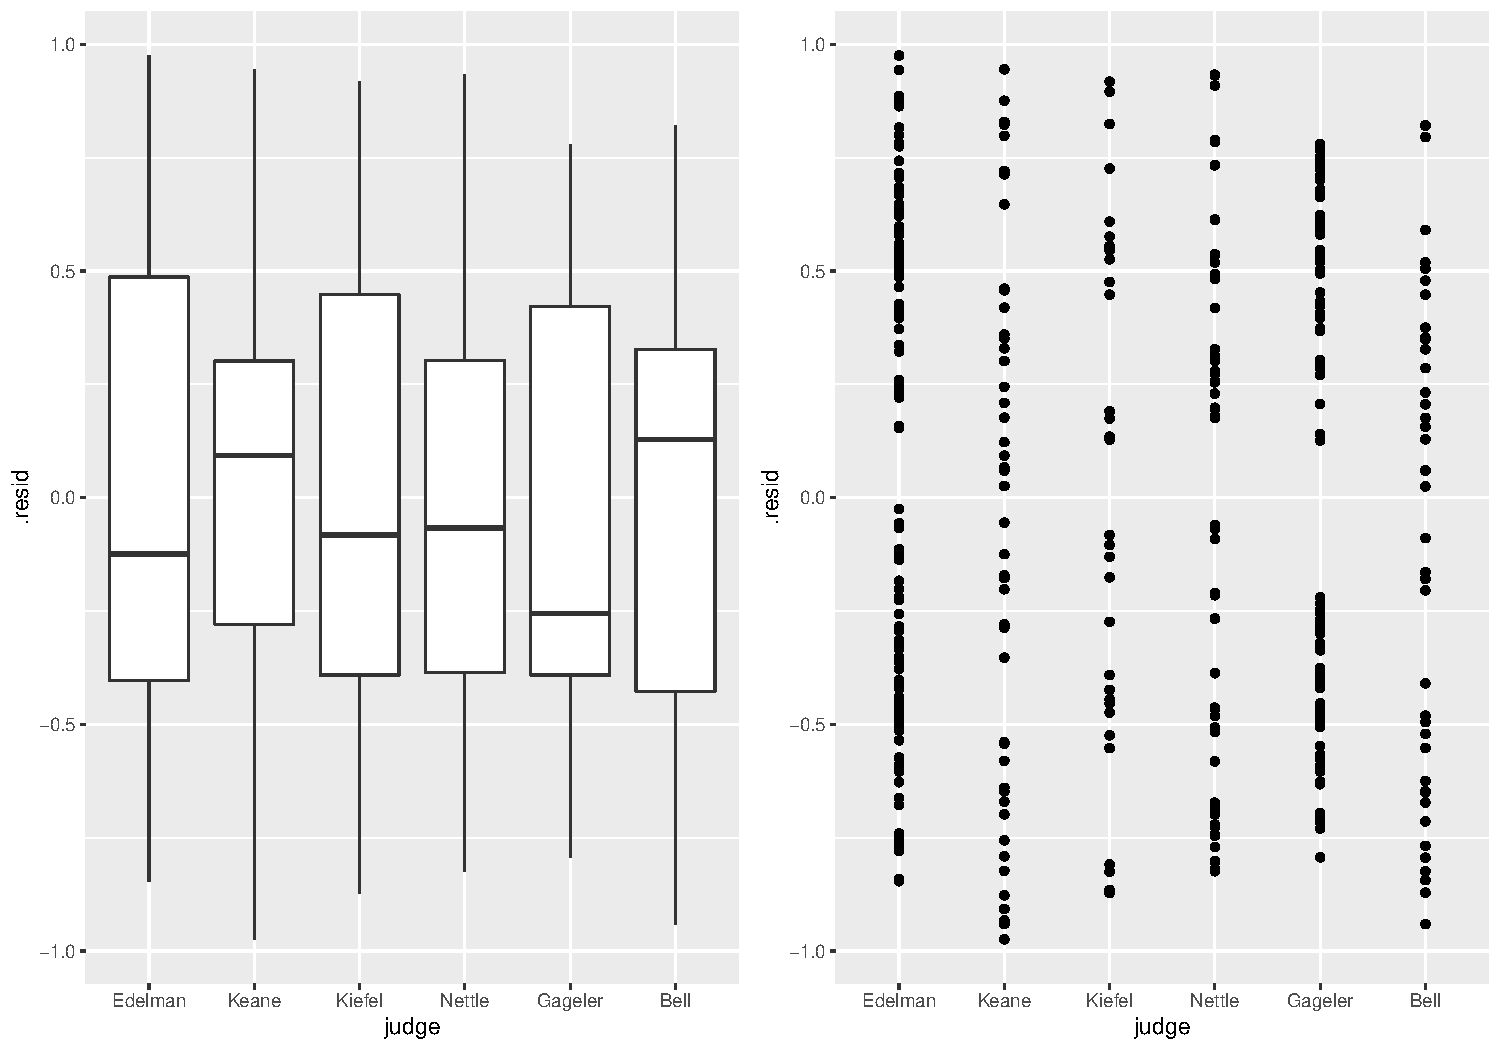
\includegraphics[width=1\linewidth]{figures/unnamed-chunk-4-1} 

}

\caption{The average presence score of each action unit for each judge, aggregating on video and time. \label{fig:mean_presence}}\label{fig:unnamed-chunk-4}
\end{figure}

\begin{table}

\caption{\label{tab:unnamed-chunk-5}\label{tab:most_common}The five most commonly presented action units for each judge.}
\centering
\begin{tabular}[t]{r|l|l|l|l|l|l}
\hline
index & Bell & Edelman & Gageler & Keane & Kiefel & Nettle\\
\hline
1 & AU15 & AU02 & AU02 & AU20 & AU02 & AU02\\
\hline
2 & AU09 & AU20 & AU05 & AU15 & AU25 & AU15\\
\hline
3 & AU25 & AU01 & AU15 & AU02 & AU45 & AU20\\
\hline
4 & AU02 & AU15 & AU14 & AU14 & AU20 & AU01\\
\hline
5 & AU01 & AU23 & AU20 & AU07 & AU14 & AU07\\
\hline
\end{tabular}
\end{table}

It can be seen that some of the action units are common across almost all the judges, these includes

\begin{itemize}
\tightlist
\item
  AU02 (outer eyebrow raise),
\item
  AU20 (lip stretcher),
\item
  AU15 (Lip Corner Depressor)
\item
  AU14 (Dimpler)
\end{itemize}

According to \textcite{ekman2002facial}, AU02 makes a contribution to surprise, which may be a positive attitude showing that judges are interested in a particular moment. AU14 indicates boredom and AU15 shows confusion. Based on the most common five action units, the emotions judges displayed in the courtroom can be summarised into three categories, described in Table \ref{tab:three_category}, along with the featured action units.

\begin{table}

\caption{\label{tab:unnamed-chunk-6}\label{tab:three_category}Summarised emotions and featured action units}
\centering
\begin{tabular}[t]{l|l}
\hline
emotion & Featured Action Unit\\
\hline
Surprise & AU01, AU02, AU05\\
\hline
Boredom & AU14, AU23\\
\hline
Confusion & AU07, AU15, AU23\\
\hline
\end{tabular}
\end{table}

\hypertarget{model-summary}{%
\subsection{Model summary}\label{model-summary}}

The estimated marginal mean is computed in Table \ref{tab:result_1} after modelling. This output can be easily interpreted as the estimated probability with its confidence interval. For example, the first row can be interpreted as follows: After averaging over all the videos and speaking parties, the estimated mean probability for judge Edelman in action unit AU02 is 0.95, with a 95\% confidence interval of {[}0.92, 0.97{]}. Notice that confidence intervals for a generalised linear model is asymmetric around the estimates because the linear symmetric interval of the mean need to be transferred via the inverse of link function to get the confidence interval for the response.

\begin{table}[ht]
\begin{center}
\caption{\label{tab:result_1}Estimated marginal mean summary for Model 1. The confidence interval is adjusted using bonferroni adjustment}
\begin{tabular}{llllll}
\toprule
judge & AU & prob & SE & asymp.LCL & asymp.UCL \\
\midrule
Edelman & AU02 & 0.95 & 0.0069 & 0.92 & 0.97 \\
Bell & AU02 & 0.73 & 0.0223 & 0.65 & 0.79 \\
Gageler & AU02 & 0.85 & 0.0125 & 0.81 & 0.89 \\
Keane & AU02 & 0.78 & 0.0207 & 0.71 & 0.84 \\
Kiefel & AU02 & 0.95 & 0.0091 & 0.91 & 0.97 \\
Nettle & AU02 & 1.00 & 0.0028 & 0.97 & 1.00 \\
Edelman & AU14 & 0.43 & 0.0155 & 0.38 & 0.48 \\
Bell & AU14 & 0.15 & 0.0179 & 0.10 & 0.22 \\
Gageler & AU14 & 0.62 & 0.0173 & 0.56 & 0.67 \\
Keane & AU14 & 0.71 & 0.0227 & 0.63 & 0.77 \\
Kiefel & AU14 & 0.52 & 0.0211 & 0.46 & 0.58 \\
Nettle & AU14 & 0.49 & 0.0201 & 0.42 & 0.55 \\
Edelman & AU15 & 0.46 & 0.0156 & 0.41 & 0.51 \\
Bell & AU15 & 0.86 & 0.0176 & 0.79 & 0.90 \\
Gageler & AU15 & 0.62 & 0.0172 & 0.57 & 0.67 \\
Keane & AU15 & 0.87 & 0.0170 & 0.80 & 0.91 \\
Kiefel & AU15 & 0.44 & 0.0210 & 0.38 & 0.51 \\
Nettle & AU15 & 0.78 & 0.0166 & 0.73 & 0.83 \\
Edelman & AU20 & 0.77 & 0.0132 & 0.72 & 0.81 \\
Bell & AU20 & 0.62 & 0.0242 & 0.55 & 0.69 \\
Gageler & AU20 & 0.55 & 0.0177 & 0.49 & 0.60 \\
Keane & AU20 & 0.93 & 0.0131 & 0.87 & 0.96 \\
Kiefel & AU20 & 0.84 & 0.0154 & 0.79 & 0.88 \\
Nettle & AU20 & 0.74 & 0.0176 & 0.68 & 0.79 \\
\bottomrule
\end{tabular}
\end{center}
\end{table}

The Type III Analysis of Variance (ANOVA) test is conducted with the result shown in Table \ref{tab:anova}. It can be seen that judge, AU and their interactions are all significance, which validates our choice of Type III instead of Type II ANOVA.

\begin{table}

\caption{\label{tab:anova}\label{tab:anova}Type III ANOVA table for model 1. All the variables are significant.}
\centering
\begin{tabular}[t]{l|l|l|l}
\hline
  & LR Chisq & Df & Pr(>Chisq)\\
\hline
judge & 319 & 5 & 8.4e-67\\
\hline
AU & 959 & 3 & 1.1e-207\\
\hline
judge:AU & 1114 & 15 & 5.1e-228\\
\hline
\end{tabular}
\end{table}

Multiple comparison is then performed and the 95\% confidence interval after bonferroni adjustment is plotted in Figure \ref{fig:model1-plot}. This plot shows that the interval for the judges are significantly different from one to another as most of the intervals are not overlapping with each other. This confirms the necessity of including the interaction terms.

\begin{figure}

{\centering 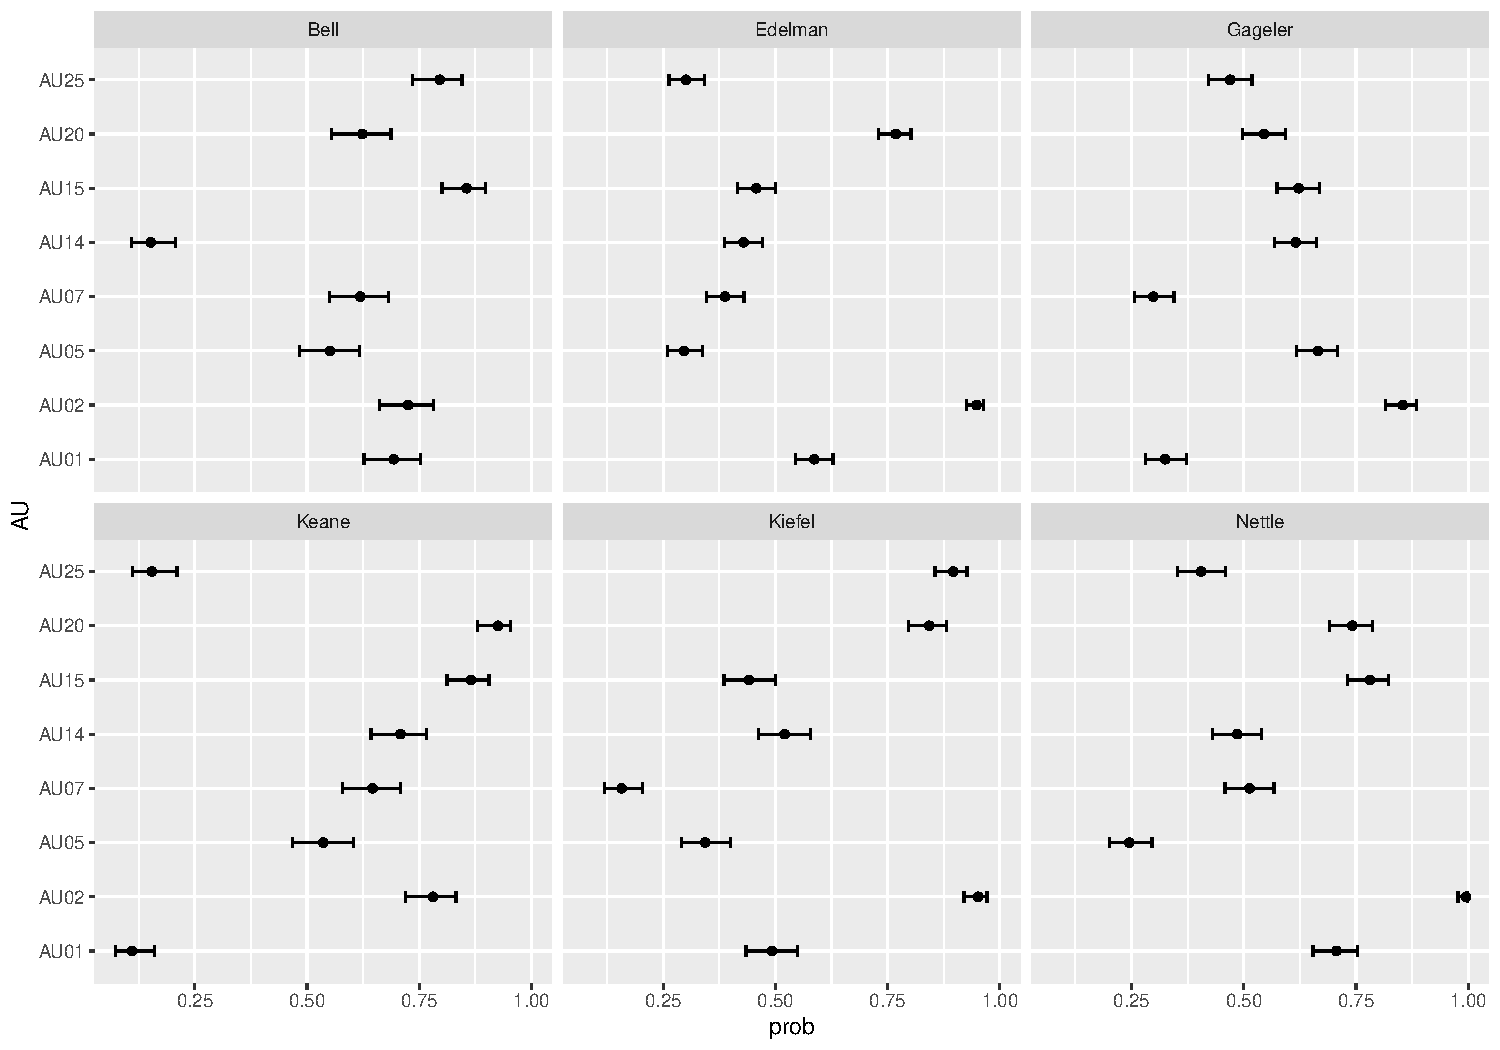
\includegraphics[width=1\linewidth]{figures/model1-plot-1} 

}

\caption{The confidence interval for estimated mearginal mean in model 1}\label{fig:model1-plot}
\end{figure}

\newpage

\hypertarget{model-2-video-1}{%
\section{Model 2: Video}\label{model-2-video-1}}

\hypertarget{presence-by-videos}{%
\subsection{Presence by videos}\label{presence-by-videos}}

We are also interested in the main presence score of the judges by video (\(P_{ijk}\)). This is computed as \[P_{ijk} = \frac{\sum_{t}X_{ijtk}}{T_j}\] for the four most common action units: AU02, AU14, AU15, AU20 and plotted in Figure \ref{fig:common_video}. From this plot, we can observe that judge Gageler, who is coloured as green, has a much higher proportion of expression in case OKS, especially in action unit 14, 15 and 20. judge Bell, who is coloured red also has large fluctuation in case Parkes for action unit 14 and 20. In the next section, I will model the presence score by incorporating the video information to see if the model tells us the same.

\begin{figure}

{\centering 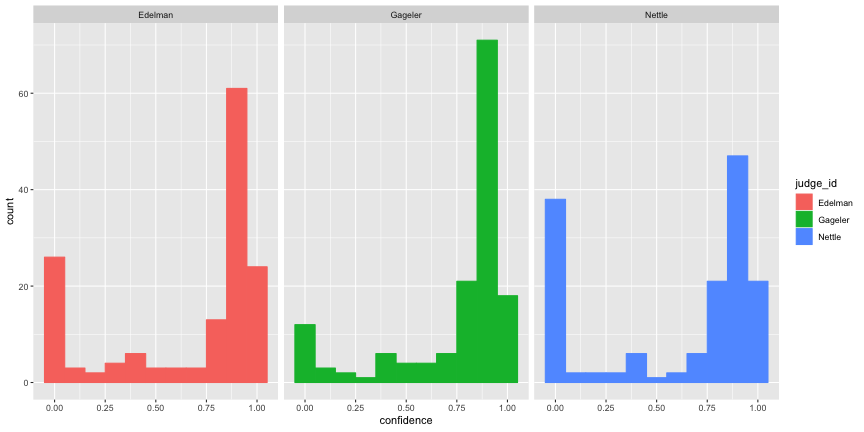
\includegraphics[width=1\linewidth]{figures/unnamed-chunk-8-1} 

}

\caption{Average presence of the four most common action units for each judge by video\label{fig:common_video}}\label{fig:unnamed-chunk-8}
\end{figure}

\hypertarget{model-summary-1}{%
\subsection{Model summary}\label{model-summary-1}}

The estimated marginal mean for the second model are presented in Table \ref{tab:result_2} in the Appendix due to its length. ANOVA test and multiple comparison is conducted as described before. Figure \ref{fig:model2-plot} presents the 95\% confidence interval for each estimated marginal mean based on model 2.

We can observe that Judge Edelman, Keane and Kiefel behave relatively consistent throughout all the videos since all the intervals overlap with each other after the bonferroni adjustment. This would indicates in these videos, these judges would have similar thinking or reaction towards the evidence and argument presented by the barristers.

Judge Gageler seems to have a large fluctuate of his facial expressions in video OKS and his response is significantly different from those in other cases for action unit 14, 15 and 20. This shows consistency with our exploratory data analysis where Gageler tends to show a higher proportion of presence for action units in case OKS.

For Judge Bell, her behaviour is much more fluctuate than all other judges. In the same Figure \ref{fig:model2-plot}, Bell shows significantly more expressions in action unit 14, 15 and 20 for case OKS and Parker, which validates the previous exploratory data analysis. From a legal perspective, this would show that Bell is addressing the cases with different responses. However, this different approach of responding by the judge doesn't indicate the biasness of the judge in the courtroom but the individuality of different judge approaching to cases.

\begin{figure}

{\centering 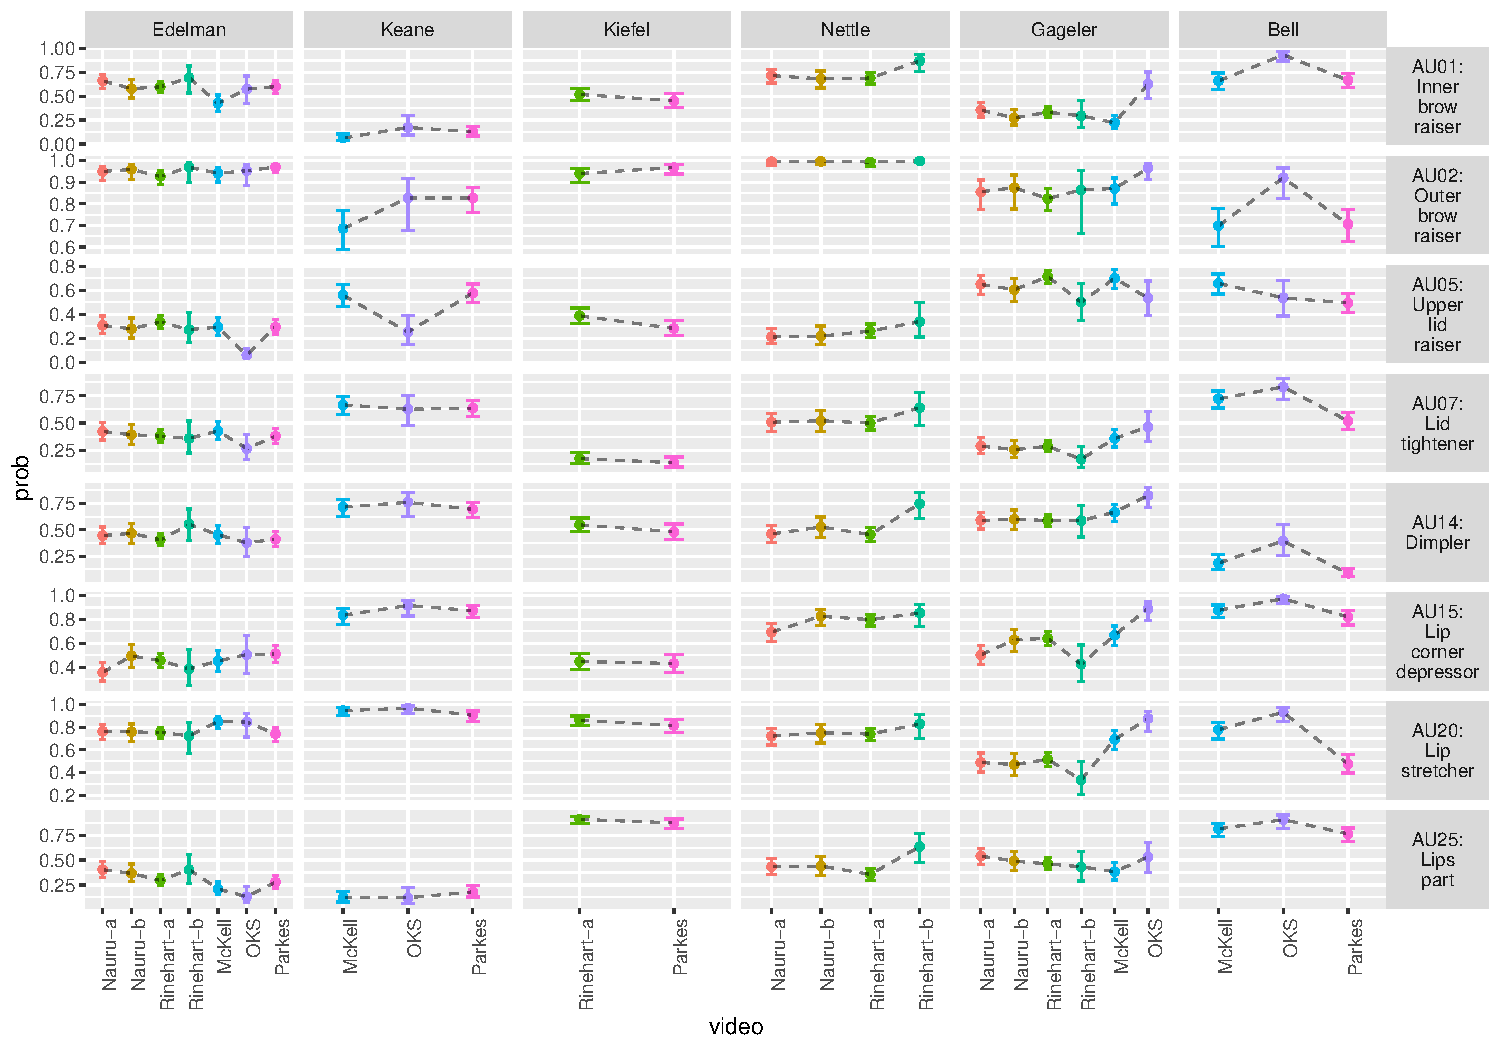
\includegraphics[width=1\linewidth]{figures/model2-plot-1} 

}

\caption{The confidence interval for estimated mearginal mean in model 2}\label{fig:model2-plot}
\end{figure}

\hypertarget{model-3-speaker-1}{%
\section{Model 3: Speaker}\label{model-3-speaker-1}}

\hypertarget{model-summary-2}{%
\subsection{Model summary}\label{model-summary-2}}

The estimated marginal mean are presented in Table \ref{tab:result_3} in the Appendix and plotted in Figure \ref{fig:model3-plot}. We can observe that the video-wise difference between judge still persist and the speaker-wise difference is not significant. This result would be a validation that on the high court level, the judges are behaving impartial to different speaking parties.

\begin{figure}

{\centering 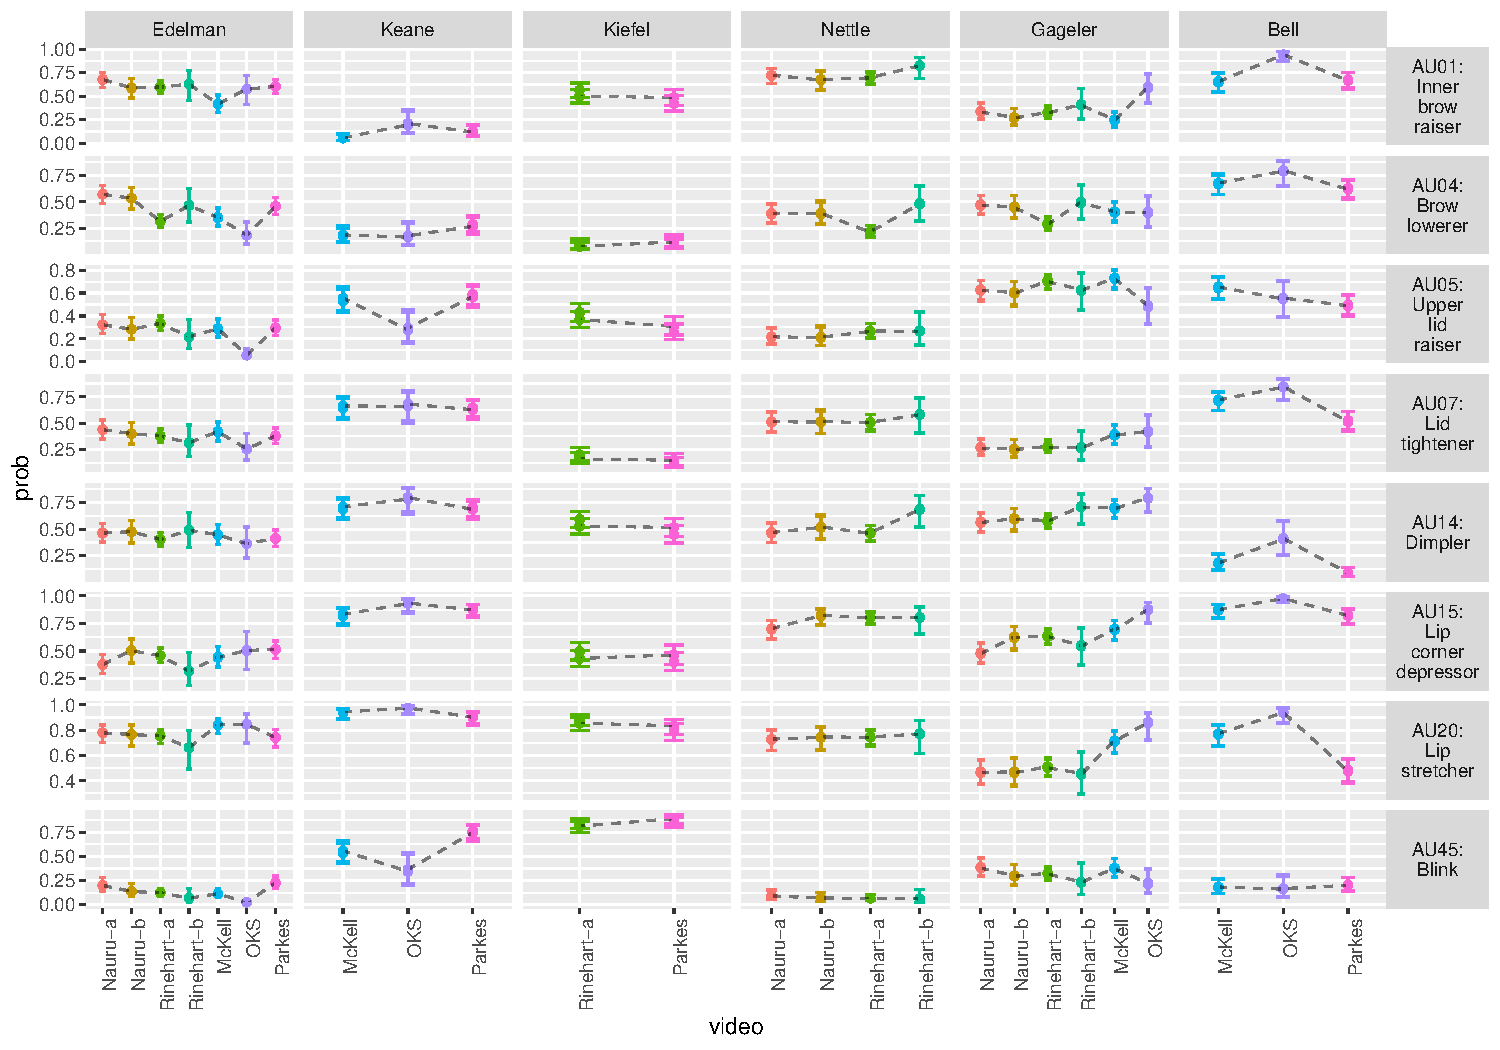
\includegraphics[width=1\linewidth]{figures/model3-plot-1} 

}

\caption{The confidence interval for estimated mearginal mean in model 3}\label{fig:model3-plot}
\end{figure}

\hypertarget{action-unit-intensity}{%
\section{Action unit: Intensity}\label{action-unit-intensity}}

\hypertarget{general-intensity-plot}{%
\subsection{General Intensity plot}\label{general-intensity-plot}}

In Ekman's 20002 FACS manual, the intensity of an action unit is defined based on five classes: Trace: 0-1, Slight: 1-2, Marked or pronounced: 2-3, Severe or extreme: 3-4 and Maximum: 4-5.

The boxplot of the intensity for all the judges across all the videos is presented in Figure \ref{fig:intensity}. Each bar-and-whisker represents the intensity (\(I_{ijtk}\)) of all the action units aggregated on time for a particular judge \(i\) in a specific case \(j\). For example, the first bar-and-whisker in case Nauru\_a is created using all the 17 action units of Edelman through out the elapsed time in Nauru\_a case.

From the plot, we can see that most of the action units have low intensity score and this is expected because usually judges are expected to behave neutral in the court room. Thus a square root transformation is taken on the y axis for better visualisation effect. We can find that Judge Nettle seems to have higher average in all the four cases he appears: Nauru\_a\&b, Rinehart\_a \&b.

\begin{figure}

{\centering 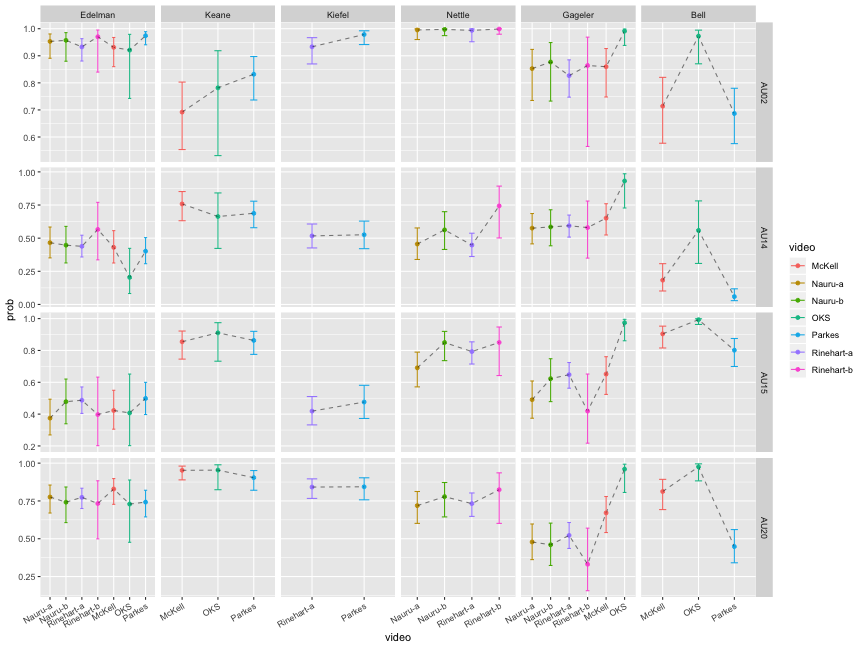
\includegraphics[width=1\linewidth]{figures/unnamed-chunk-10-1} 

}

\caption{General intensity score by judge and video\label{fig:intensity}}\label{fig:unnamed-chunk-10}
\end{figure}

\hypertarget{mean-intensity}{%
\subsection{Mean intensity}\label{mean-intensity}}

Mean intensity score (\(I_{ik}\)) of each action unit for each of the judge is computed as \[I_{ik} = \frac{\sum_{jt}X_{ijtk}}{\sum_{j = 1}^JT_j}\] and plotted in Figure \ref{fig:mean_intensity}. The five most intense action units for each judge are presented in Table \ref{tab:most_intense}. We can find that the common high intense action units includes

\begin{itemize}
\tightlist
\item
  AU20 (Lip Stretcher)
\item
  AU07 (Lid Tightener)
\item
  AU04 (Brow Lower)
\end{itemize}

AU04 also belongs to the confusion category as AU07. This could help to understand that judges are more likely to express a stronger confusing expression than other emotions.

\begin{figure}

{\centering 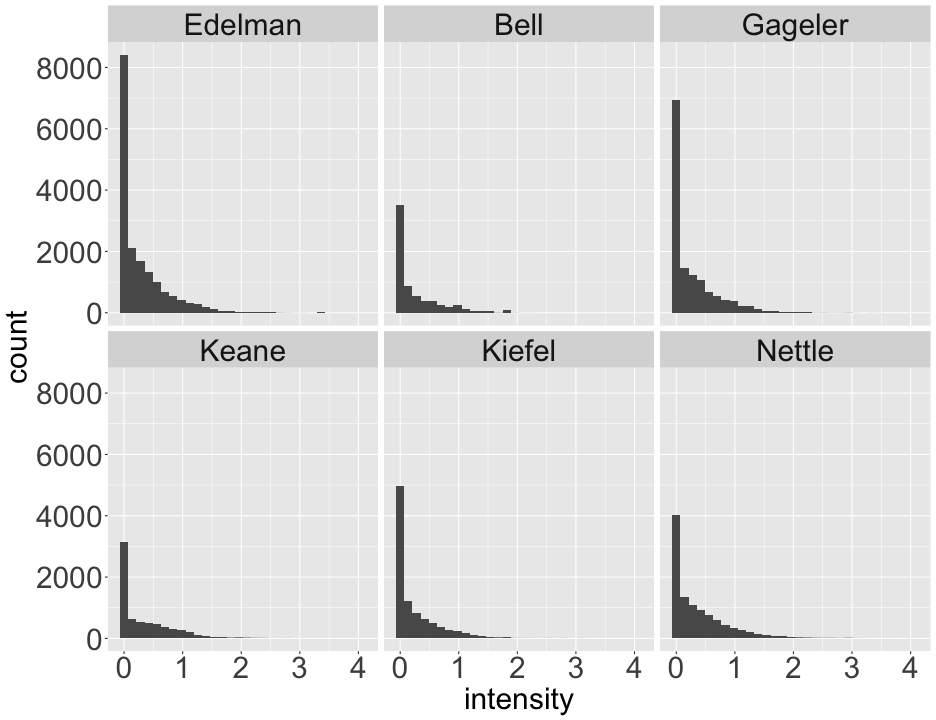
\includegraphics[width=1\linewidth]{figures/unnamed-chunk-12-1} 

}

\caption{Mean intensity score for each judge and action unit aggregating on videos.\label{fig:mean_intensity}}\label{fig:unnamed-chunk-12}
\end{figure}

\begin{table}

\caption{\label{tab:unnamed-chunk-13}\label{tab:most_intense}The five most intense action unit for each judge.}
\centering
\begin{tabular}[t]{r|l|l|l|l|l|l}
\hline
index & Bell & Edelman & Gageler & Keane & Kiefel & Nettle\\
\hline
1 & AU04 & AU20 & AU05 & AU20 & AU45 & AU20\\
\hline
2 & AU09 & AU06 & AU04 & AU07 & AU20 & AU01\\
\hline
3 & AU07 & AU17 & AU20 & AU15 & AU26 & AU07\\
\hline
4 & AU15 & AU07 & AU09 & AU14 & AU25 & AU06\\
\hline
5 & AU10 & AU04 & AU45 & AU17 & AU14 & AU17\\
\hline
\end{tabular}
\end{table}

\hypertarget{model-fit}{%
\subsection{Model fit}\label{model-fit}}

\hypertarget{intensity-plot-for-the-most-frequent-action-units}{%
\subsection{Intensity plot for the most frequent action units}\label{intensity-plot-for-the-most-frequent-action-units}}

Apart from visualising the general intensity score for all the action units, I'm also interested in the intensity score of the most frequent action units. Figure \ref{fig:intensity_by_au} presents this. The statistics being plotted is \(I_{ijtk}\) with \(k\) including AU02, AU14, AU15 and AU20 as the most common four action units. From this plot, we can learn that AU02, although being commonly detected for all the judges, has low intensity score.

\begin{figure}

{\centering \includegraphics[width=1\linewidth]{figures/unnamed-chunk-15-1} 

}

\caption{Intensity score of the most frequent action units, seperating by judge and video ID.\label{fig:intensity_by_au}}\label{fig:unnamed-chunk-15}
\end{figure}

\hypertarget{high-intensity-points}{%
\subsection{High intensity points}\label{high-intensity-points}}

We filter out the points have intensity greater than 2 (at least ``slight'' as per Ekman) in the previous plot and plot it against time and color by the speaker. It tells us that Edelman, Gageler and Nettle are the judges have stronger emotion that can be detected (since they have more points with intensity greater than 2). Different judges also have different time where they display stronger emotions. For example, Justice Nettle are more likely to have stronger emotion throughout the time when the appellant is speaking but only at the beginning and ending period when the respondent is speaking.

\begin{center}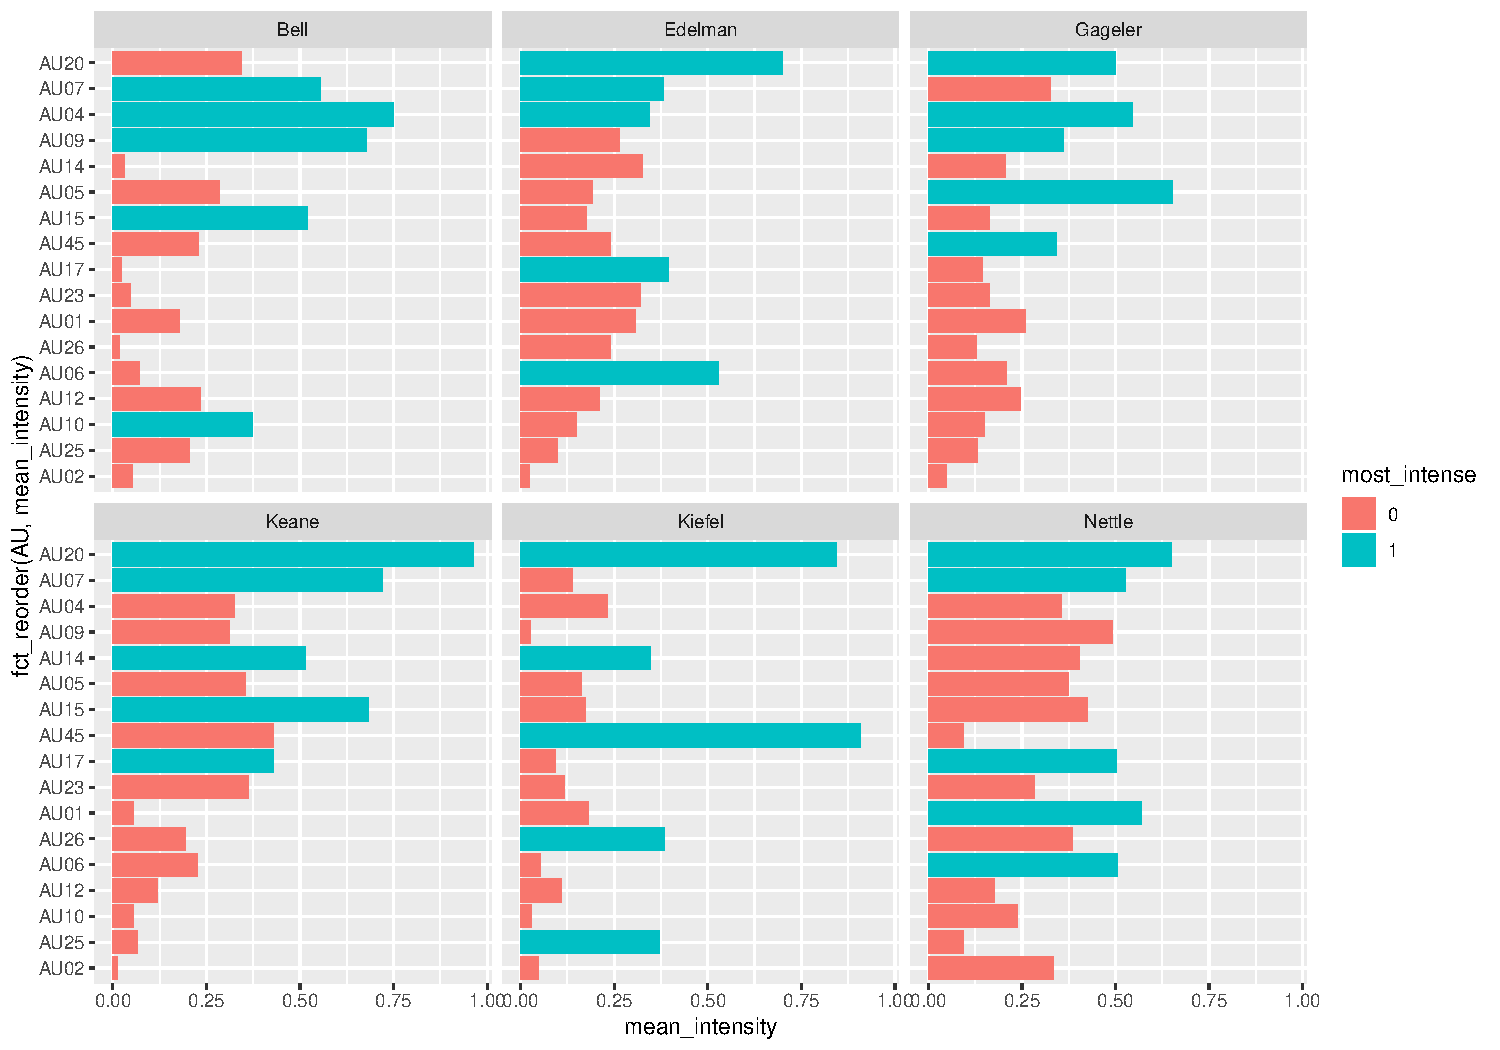
\includegraphics[width=1\linewidth]{figures/unnamed-chunk-16-1} \end{center}

\hypertarget{conclusion}{%
\chapter{Conclusion}\label{conclusion}}

\hypertarget{discussion}{%
\section{Discussion}\label{discussion}}

\hypertarget{limitation}{%
\section{Limitation}\label{limitation}}

I will now briefly discuss some of the limitation of this work. The current image frames are extracted at every one minute interval. However, some facial expressions may only last for a few second. Thus more frequent time interval could be used for getting more precise facial information of the judges.

In my work, seven videos are being processed into the facial recognition software and more videos could be processed to get more robust results. The reason for not processing more videos in the current study is because the resolution of publicly available vidoes from the high court has only 720 pixels while the facial recognition software, OpenFace requires at least 30 pixels for a face to be detected. This means that we have to choose videos where three or five judges are presented.

However, this work has established a workflow for extracting facial expressions of human from videos. As long as more higher resolution videos are available, facial variables can be extracted via the same fashion.

\hypertarget{future-work}{%
\section{Future work}\label{future-work}}

\appendix

\hypertarget{appendix}{%
\chapter{Appendix}\label{appendix}}

\hypertarget{list-of-videos-used-in-the-project}{%
\section{List of videos used in the project}\label{list-of-videos-used-in-the-project}}

\begin{longtable}[]{@{}llll@{}}
\caption{Details of videos processed.}\tabularnewline
\toprule
\begin{minipage}[b]{0.22\columnwidth}\raggedright
Case\strut
\end{minipage} & \begin{minipage}[b]{0.15\columnwidth}\raggedright
Name\strut
\end{minipage} & \begin{minipage}[b]{0.30\columnwidth}\raggedright
AV recording link\strut
\end{minipage} & \begin{minipage}[b]{0.22\columnwidth}\raggedright
Judge\strut
\end{minipage}\tabularnewline
\midrule
\endfirsthead
\toprule
\begin{minipage}[b]{0.22\columnwidth}\raggedright
Case\strut
\end{minipage} & \begin{minipage}[b]{0.15\columnwidth}\raggedright
Name\strut
\end{minipage} & \begin{minipage}[b]{0.30\columnwidth}\raggedright
AV recording link\strut
\end{minipage} & \begin{minipage}[b]{0.22\columnwidth}\raggedright
Judge\strut
\end{minipage}\tabularnewline
\midrule
\endhead
\begin{minipage}[t]{0.22\columnwidth}\raggedright
The Republic of Nauru v WET040 {[}No.~2{]} {[}2018{]} HCA 60\strut
\end{minipage} & \begin{minipage}[t]{0.15\columnwidth}\raggedright
\texttt{Nauru\_a}\strut
\end{minipage} & \begin{minipage}[t]{0.30\columnwidth}\raggedright
\url{http://www.hcourt.gov.au/cases/cases-av/av-2018-11-07a}\strut
\end{minipage} & \begin{minipage}[t]{0.22\columnwidth}\raggedright
Nettle, Gageler, Edelman\strut
\end{minipage}\tabularnewline
\begin{minipage}[t]{0.22\columnwidth}\raggedright
TTY167 v Republic of Nauru {[}2018{]} HCA 61\strut
\end{minipage} & \begin{minipage}[t]{0.15\columnwidth}\raggedright
\texttt{Nauru\_b}\strut
\end{minipage} & \begin{minipage}[t]{0.30\columnwidth}\raggedright
\url{http://www.hcourt.gov.au/cases/cases-av/av-2018-11-07b}\strut
\end{minipage} & \begin{minipage}[t]{0.22\columnwidth}\raggedright
Nettle, Gageler, Edelman\strut
\end{minipage}\tabularnewline
\begin{minipage}[t]{0.22\columnwidth}\raggedright
Rinehart v Hancock Prospecting Pty Ltd {[}2019{]} HCA 13\strut
\end{minipage} & \begin{minipage}[t]{0.15\columnwidth}\raggedright
\texttt{Rinehart\_a}\strut
\end{minipage} & \begin{minipage}[t]{0.30\columnwidth}\raggedright
\url{http://www.hcourt.gov.au/cases/cases-av/av-2018-11-13}\strut
\end{minipage} & \begin{minipage}[t]{0.22\columnwidth}\raggedright
Gordon, Gageler, Bell, Keane, Edelman\strut
\end{minipage}\tabularnewline
\begin{minipage}[t]{0.22\columnwidth}\raggedright
Rinehart v Hancock Prospecting Pty Ltd {[}2019{]} HCA 13\strut
\end{minipage} & \begin{minipage}[t]{0.15\columnwidth}\raggedright
\texttt{Rinehart\_b}\strut
\end{minipage} & \begin{minipage}[t]{0.30\columnwidth}\raggedright
\url{http://www.hcourt.gov.au/cases/cases-av/av-2018-11-14a}\strut
\end{minipage} & \begin{minipage}[t]{0.22\columnwidth}\raggedright
Gordon, Keane, Bell, Gageler, Edelman\strut
\end{minipage}\tabularnewline
\begin{minipage}[t]{0.22\columnwidth}\raggedright
Parkes Shire Council v South West Helicopters Pty Limited {[}2019{]} HCA 14\strut
\end{minipage} & \begin{minipage}[t]{0.15\columnwidth}\raggedright
\texttt{Parkes}\strut
\end{minipage} & \begin{minipage}[t]{0.30\columnwidth}\raggedright
\url{http://www.hcourt.gov.au/cases/cases-av/av-2018-11-14b}\strut
\end{minipage} & \begin{minipage}[t]{0.22\columnwidth}\raggedright
Gordon, Bell, Kiefel, Keane, Edelman\strut
\end{minipage}\tabularnewline
\begin{minipage}[t]{0.22\columnwidth}\raggedright
McKell v The Queen {[}2019{]} HCA 5\strut
\end{minipage} & \begin{minipage}[t]{0.15\columnwidth}\raggedright
\texttt{McKell}\strut
\end{minipage} & \begin{minipage}[t]{0.30\columnwidth}\raggedright
\url{http://www.hcourt.gov.au/cases/cases-av/av-2018-12-07}\strut
\end{minipage} & \begin{minipage}[t]{0.22\columnwidth}\raggedright
Gordon, Gageler, Kiefel, Nettle, Edelman\strut
\end{minipage}\tabularnewline
\begin{minipage}[t]{0.22\columnwidth}\raggedright
OKS v Western Australia {[}2019{]} HCA 10\strut
\end{minipage} & \begin{minipage}[t]{0.15\columnwidth}\raggedright
\texttt{OKS}\strut
\end{minipage} & \begin{minipage}[t]{0.30\columnwidth}\raggedright
\url{http://www.hcourt.gov.au/cases/cases-av/av-2019-02-14}\strut
\end{minipage} & \begin{minipage}[t]{0.22\columnwidth}\raggedright
Gordon, Gageler, Kiefel, Nettle, Edelman\strut
\end{minipage}\tabularnewline
\bottomrule
\end{longtable}

\hypertarget{list-of-the-name-of-ction-units}{%
\section{List of the name of ction units}\label{list-of-the-name-of-ction-units}}

\begin{table}[ht]
\begin{center}
\caption{\label{tab:au_meaning} The meaning of all the action unit estimated}
\begin{tabular}{l}
\toprule
AU-meaning \\
\midrule
AU01: Inner brow raiser \\
AU02: Outer brow raiser \\
AU04: Brow lowerer \\
AU05: Upper lid raiser \\
AU06: Cheek raiser \\
AU07: Lid tightener \\
AU09: Nose wrinkler \\
AU10: Upper lip raiser \\
AU12: Lip corner puller \\
AU14: Dimpler \\
AU15: Lip corner depressor \\
AU17: Chin raiser \\
AU20: Lip stretcher \\
AU23: Lip tightener \\
AU25: Lips part \\
AU26: Jaw drop \\
AU28: Lip suck \\
AU45: Blink \\
\bottomrule
\end{tabular}
\end{center}
\end{table}

\hypertarget{model-estimation-result}{%
\section{Model estimation result}\label{model-estimation-result}}

\begin{center}
\begin{longtable}{lllllll}
\caption{\label{tab:result_2} model result 2}\\
\toprule
judge & video & AU & prob & SE & asymp.LCL & asymp.UCL \\
\midrule
\endhead
\bottomrule
\endfoot
Edelman & McKell & AU02 & 0.931 & 0.01401 & 0.883 & 0.961 \\
Bell & McKell & AU02 & 0.714 & 0.03411 & 0.614 & 0.796 \\
Gageler & McKell & AU02 & 0.860 & 0.02419 & 0.781 & 0.913 \\
Keane & McKell & AU02 & 0.692 & 0.03503 & 0.591 & 0.778 \\
Edelman & Nauru-a & AU02 & 0.953 & 0.01127 & 0.912 & 0.976 \\
Gageler & Nauru-a & AU02 & 0.853 & 0.02556 & 0.770 & 0.909 \\
Nettle & Nauru-a & AU02 & 0.995 & 0.00275 & 0.977 & 0.999 \\
Edelman & Nauru-b & AU02 & 0.957 & 0.01263 & 0.907 & 0.981 \\
Gageler & Nauru-b & AU02 & 0.877 & 0.02850 & 0.778 & 0.936 \\
Nettle & Nauru-b & AU02 & 0.998 & 0.00161 & 0.986 & 1.000 \\
Edelman & OKS & AU02 & 0.921 & 0.02810 & 0.805 & 0.971 \\
Bell & OKS & AU02 & 0.973 & 0.01224 & 0.912 & 0.992 \\
Gageler & OKS & AU02 & 0.991 & 0.00482 & 0.962 & 0.998 \\
Keane & OKS & AU02 & 0.782 & 0.05426 & 0.604 & 0.894 \\
Edelman & Parkes & AU02 & 0.974 & 0.00603 & 0.952 & 0.986 \\
Bell & Parkes & AU02 & 0.687 & 0.02858 & 0.605 & 0.758 \\
Keane & Parkes & AU02 & 0.832 & 0.02202 & 0.764 & 0.883 \\
Kiefel & Parkes & AU02 & 0.979 & 0.00604 & 0.955 & 0.990 \\
Edelman & Rinehart-a & AU02 & 0.933 & 0.01095 & 0.897 & 0.957 \\
Gageler & Rinehart-a & AU02 & 0.827 & 0.01894 & 0.770 & 0.872 \\
Kiefel & Rinehart-a & AU02 & 0.933 & 0.01271 & 0.890 & 0.960 \\
Nettle & Rinehart-a & AU02 & 0.994 & 0.00353 & 0.971 & 0.999 \\
Edelman & Rinehart-b & AU02 & 0.970 & 0.01455 & 0.893 & 0.992 \\
Gageler & Rinehart-b & AU02 & 0.864 & 0.05155 & 0.661 & 0.954 \\
Nettle & Rinehart-b & AU02 & 0.999 & 0.00095 & 0.990 & 1.000 \\
Edelman & McKell & AU14 & 0.431 & 0.03440 & 0.341 & 0.524 \\
Bell & McKell & AU14 & 0.183 & 0.02830 & 0.119 & 0.271 \\
Gageler & McKell & AU14 & 0.651 & 0.03312 & 0.558 & 0.734 \\
Keane & McKell & AU14 & 0.758 & 0.03063 & 0.667 & 0.831 \\
Edelman & Nauru-a & AU14 & 0.466 & 0.03275 & 0.380 & 0.554 \\
Gageler & Nauru-a & AU14 & 0.575 & 0.03218 & 0.487 & 0.659 \\
Nettle & Nauru-a & AU14 & 0.456 & 0.03350 & 0.368 & 0.546 \\
Edelman & Nauru-b & AU14 & 0.447 & 0.03911 & 0.346 & 0.553 \\
Gageler & Nauru-b & AU14 & 0.585 & 0.03848 & 0.479 & 0.683 \\
Nettle & Nauru-b & AU14 & 0.562 & 0.04047 & 0.452 & 0.667 \\
Edelman & OKS & AU14 & 0.204 & 0.04718 & 0.105 & 0.359 \\
Bell & OKS & AU14 & 0.558 & 0.07074 & 0.369 & 0.732 \\
Gageler & OKS & AU14 & 0.931 & 0.02873 & 0.802 & 0.978 \\
Keane & OKS & AU14 & 0.663 & 0.06109 & 0.486 & 0.804 \\
Edelman & Parkes & AU14 & 0.402 & 0.02753 & 0.330 & 0.477 \\
Bell & Parkes & AU14 & 0.059 & 0.01160 & 0.035 & 0.099 \\
Keane & Parkes & AU14 & 0.687 & 0.02796 & 0.608 & 0.757 \\
Kiefel & Parkes & AU14 & 0.526 & 0.02919 & 0.447 & 0.603 \\
Edelman & Rinehart-a & AU14 & 0.438 & 0.02287 & 0.378 & 0.501 \\
Gageler & Rinehart-a & AU14 & 0.594 & 0.02316 & 0.530 & 0.654 \\
Kiefel & Rinehart-a & AU14 & 0.517 & 0.02524 & 0.449 & 0.584 \\
Nettle & Rinehart-a & AU14 & 0.448 & 0.02456 & 0.383 & 0.514 \\
Edelman & Rinehart-b & AU14 & 0.566 & 0.06411 & 0.392 & 0.725 \\
Gageler & Rinehart-b & AU14 & 0.580 & 0.06352 & 0.406 & 0.736 \\
Nettle & Rinehart-b & AU14 & 0.743 & 0.05574 & 0.569 & 0.864 \\
Edelman & McKell & AU15 & 0.423 & 0.03445 & 0.334 & 0.517 \\
Bell & McKell & AU15 & 0.904 & 0.01816 & 0.843 & 0.943 \\
Gageler & McKell & AU15 & 0.652 & 0.03329 & 0.558 & 0.735 \\
Keane & McKell & AU15 & 0.855 & 0.02392 & 0.778 & 0.908 \\
Edelman & Nauru-a & AU15 & 0.375 & 0.03152 & 0.294 & 0.463 \\
Gageler & Nauru-a & AU15 & 0.491 & 0.03294 & 0.403 & 0.579 \\
Nettle & Nauru-a & AU15 & 0.691 & 0.03057 & 0.603 & 0.767 \\
Edelman & Nauru-b & AU15 & 0.478 & 0.03990 & 0.373 & 0.585 \\
Gageler & Nauru-b & AU15 & 0.623 & 0.03813 & 0.516 & 0.719 \\
Nettle & Nauru-b & AU15 & 0.850 & 0.02498 & 0.770 & 0.905 \\
Edelman & OKS & AU15 & 0.407 & 0.06677 & 0.246 & 0.591 \\
Bell & OKS & AU15 & 0.993 & 0.00319 & 0.976 & 0.998 \\
Gageler & OKS & AU15 & 0.974 & 0.01259 & 0.908 & 0.993 \\
Keane & OKS & AU15 & 0.911 & 0.02957 & 0.793 & 0.965 \\
Edelman & Parkes & AU15 & 0.498 & 0.02836 & 0.423 & 0.574 \\
Bell & Parkes & AU15 & 0.801 & 0.02427 & 0.728 & 0.859 \\
Keane & Parkes & AU15 & 0.863 & 0.01969 & 0.801 & 0.908 \\
Kiefel & Parkes & AU15 & 0.476 & 0.02923 & 0.398 & 0.554 \\
Edelman & Rinehart-a & AU15 & 0.487 & 0.02319 & 0.425 & 0.549 \\
Gageler & Rinehart-a & AU15 & 0.648 & 0.02246 & 0.585 & 0.705 \\
Kiefel & Rinehart-a & AU15 & 0.419 & 0.02488 & 0.354 & 0.487 \\
Nettle & Rinehart-a & AU15 & 0.793 & 0.01925 & 0.736 & 0.840 \\
Edelman & Rinehart-b & AU15 & 0.397 & 0.06348 & 0.244 & 0.574 \\
Gageler & Rinehart-b & AU15 & 0.419 & 0.06417 & 0.262 & 0.594 \\
Nettle & Rinehart-b & AU15 & 0.850 & 0.04053 & 0.707 & 0.930 \\
Edelman & McKell & AU20 & 0.829 & 0.02334 & 0.757 & 0.883 \\
Bell & McKell & AU20 & 0.813 & 0.02751 & 0.727 & 0.876 \\
Gageler & McKell & AU20 & 0.671 & 0.03347 & 0.576 & 0.754 \\
Keane & McKell & AU20 & 0.953 & 0.01143 & 0.910 & 0.975 \\
Edelman & Nauru-a & AU20 & 0.776 & 0.02562 & 0.700 & 0.837 \\
Gageler & Nauru-a & AU20 & 0.479 & 0.03319 & 0.391 & 0.568 \\
Nettle & Nauru-a & AU20 & 0.719 & 0.02943 & 0.634 & 0.791 \\
Edelman & Nauru-b & AU20 & 0.742 & 0.03287 & 0.644 & 0.820 \\
Gageler & Nauru-b & AU20 & 0.460 & 0.03976 & 0.357 & 0.567 \\
Nettle & Nauru-b & AU20 & 0.778 & 0.03157 & 0.682 & 0.852 \\
Edelman & OKS & AU20 & 0.729 & 0.05918 & 0.546 & 0.858 \\
Bell & OKS & AU20 & 0.976 & 0.01098 & 0.920 & 0.993 \\
Gageler & OKS & AU20 & 0.960 & 0.01853 & 0.867 & 0.989 \\
Keane & OKS & AU20 & 0.954 & 0.01806 & 0.873 & 0.984 \\
Edelman & Parkes & AU20 & 0.742 & 0.02448 & 0.671 & 0.803 \\
Bell & Parkes & AU20 & 0.448 & 0.03085 & 0.367 & 0.532 \\
Keane & Parkes & AU20 & 0.904 & 0.01730 & 0.846 & 0.942 \\
Kiefel & Parkes & AU20 & 0.844 & 0.01992 & 0.782 & 0.890 \\
Edelman & Rinehart-a & AU20 & 0.774 & 0.01857 & 0.720 & 0.820 \\
Gageler & Rinehart-a & AU20 & 0.522 & 0.02394 & 0.458 & 0.586 \\
Kiefel & Rinehart-a & AU20 & 0.842 & 0.01775 & 0.788 & 0.884 \\
Nettle & Rinehart-a & AU20 & 0.732 & 0.02151 & 0.671 & 0.786 \\
Edelman & Rinehart-b & AU20 & 0.733 & 0.05482 & 0.564 & 0.854 \\
Gageler & Rinehart-b & AU20 & 0.331 & 0.06028 & 0.193 & 0.508 \\
Nettle & Rinehart-b & AU20 & 0.824 & 0.04538 & 0.669 & 0.916 \\
\end{longtable}
\end{center}

\begin{center}
\begin{longtable}{llllllll}
\caption{\label{tab:result_3} model result 3}\\
\toprule
judge & video & AU & speaker & prob & SE & asymp.LCL & asymp.UCL \\
\midrule
\endhead
\bottomrule
\endfoot
Edelman & McKell & AU02 & Appellent & 0.930 & 0.0143 & 0.875 & 0.962 \\
Bell & McKell & AU02 & Appellent & 0.697 & 0.0363 & 0.583 & 0.792 \\
Gageler & McKell & AU02 & Appellent & 0.858 & 0.0247 & 0.770 & 0.916 \\
Keane & McKell & AU02 & Appellent & 0.679 & 0.0371 & 0.563 & 0.776 \\
Edelman & Nauru-a & AU02 & Appellent & 0.952 & 0.0115 & 0.905 & 0.977 \\
Gageler & Nauru-a & AU02 & Appellent & 0.850 & 0.0263 & 0.757 & 0.912 \\
Nettle & Nauru-a & AU02 & Appellent & 0.996 & 0.0026 & 0.975 & 0.999 \\
Edelman & Nauru-b & AU02 & Appellent & 0.957 & 0.0127 & 0.901 & 0.982 \\
Gageler & Nauru-b & AU02 & Appellent & 0.876 & 0.0286 & 0.766 & 0.939 \\
Nettle & Nauru-b & AU02 & Appellent & 0.998 & 0.0016 & 0.984 & 1.000 \\
Edelman & OKS & AU02 & Appellent & 0.920 & 0.0287 & 0.787 & 0.973 \\
Bell & OKS & AU02 & Appellent & 0.970 & 0.0137 & 0.891 & 0.992 \\
Gageler & OKS & AU02 & Appellent & 0.991 & 0.0049 & 0.956 & 0.998 \\
Keane & OKS & AU02 & Appellent & 0.766 & 0.0581 & 0.560 & 0.894 \\
Edelman & Parkes & AU02 & Appellent & 0.974 & 0.0063 & 0.947 & 0.987 \\
Bell & Parkes & AU02 & Appellent & 0.651 & 0.0358 & 0.541 & 0.747 \\
Keane & Parkes & AU02 & Appellent & 0.814 & 0.0272 & 0.722 & 0.881 \\
Kiefel & Parkes & AU02 & Appellent & 0.984 & 0.0048 & 0.962 & 0.993 \\
Edelman & Rinehart-a & AU02 & Appellent & 0.931 & 0.0117 & 0.888 & 0.958 \\
Gageler & Rinehart-a & AU02 & Appellent & 0.822 & 0.0209 & 0.753 & 0.875 \\
Kiefel & Rinehart-a & AU02 & Appellent & 0.949 & 0.0106 & 0.908 & 0.972 \\
Nettle & Rinehart-a & AU02 & Appellent & 0.994 & 0.0032 & 0.970 & 0.999 \\
Edelman & Rinehart-b & AU02 & Appellent & 0.970 & 0.0148 & 0.881 & 0.993 \\
Gageler & Rinehart-b & AU02 & Appellent & 0.862 & 0.0523 & 0.635 & 0.958 \\
Nettle & Rinehart-b & AU02 & Appellent & 0.999 & 0.0009 & 0.989 & 1.000 \\
Edelman & McKell & AU14 & Appellent & 0.427 & 0.0349 & 0.330 & 0.530 \\
Bell & McKell & AU14 & Appellent & 0.170 & 0.0276 & 0.104 & 0.266 \\
Gageler & McKell & AU14 & Appellent & 0.647 & 0.0339 & 0.544 & 0.739 \\
Keane & McKell & AU14 & Appellent & 0.747 & 0.0326 & 0.641 & 0.830 \\
Edelman & Nauru-a & AU14 & Appellent & 0.461 & 0.0337 & 0.366 & 0.560 \\
Gageler & Nauru-a & AU14 & Appellent & 0.570 & 0.0334 & 0.472 & 0.664 \\
Nettle & Nauru-a & AU14 & Appellent & 0.470 & 0.0355 & 0.369 & 0.573 \\
Edelman & Nauru-b & AU14 & Appellent & 0.446 & 0.0392 & 0.336 & 0.561 \\
Gageler & Nauru-b & AU14 & Appellent & 0.583 & 0.0386 & 0.468 & 0.690 \\
Nettle & Nauru-b & AU14 & Appellent & 0.567 & 0.0405 & 0.447 & 0.679 \\
Edelman & OKS & AU14 & Appellent & 0.201 & 0.0470 & 0.097 & 0.371 \\
Bell & OKS & AU14 & Appellent & 0.528 & 0.0733 & 0.322 & 0.725 \\
Gageler & OKS & AU14 & Appellent & 0.930 & 0.0294 & 0.781 & 0.980 \\
Keane & OKS & AU14 & Appellent & 0.643 & 0.0646 & 0.442 & 0.803 \\
Edelman & Parkes & AU14 & Appellent & 0.395 & 0.0300 & 0.312 & 0.485 \\
Bell & Parkes & AU14 & Appellent & 0.050 & 0.0109 & 0.026 & 0.093 \\
Keane & Parkes & AU14 & Appellent & 0.660 & 0.0352 & 0.552 & 0.754 \\
Kiefel & Parkes & AU14 & Appellent & 0.593 & 0.0332 & 0.493 & 0.685 \\
Edelman & Rinehart-a & AU14 & Appellent & 0.432 & 0.0260 & 0.358 & 0.509 \\
Gageler & Rinehart-a & AU14 & Appellent & 0.586 & 0.0268 & 0.507 & 0.661 \\
Kiefel & Rinehart-a & AU14 & Appellent & 0.584 & 0.0301 & 0.494 & 0.668 \\
Nettle & Rinehart-a & AU14 & Appellent & 0.471 & 0.0305 & 0.384 & 0.559 \\
Edelman & Rinehart-b & AU14 & Appellent & 0.562 & 0.0646 & 0.374 & 0.734 \\
Gageler & Rinehart-b & AU14 & Appellent & 0.576 & 0.0641 & 0.387 & 0.745 \\
Nettle & Rinehart-b & AU14 & Appellent & 0.752 & 0.0549 & 0.563 & 0.878 \\
Edelman & McKell & AU15 & Appellent & 0.419 & 0.0349 & 0.322 & 0.523 \\
Bell & McKell & AU15 & Appellent & 0.897 & 0.0196 & 0.824 & 0.942 \\
Gageler & McKell & AU15 & Appellent & 0.648 & 0.0340 & 0.544 & 0.740 \\
Keane & McKell & AU15 & Appellent & 0.847 & 0.0255 & 0.757 & 0.908 \\
Edelman & Nauru-a & AU15 & Appellent & 0.371 & 0.0323 & 0.282 & 0.469 \\
Gageler & Nauru-a & AU15 & Appellent & 0.486 & 0.0341 & 0.388 & 0.584 \\
Nettle & Nauru-a & AU15 & Appellent & 0.704 & 0.0315 & 0.605 & 0.786 \\
Edelman & Nauru-b & AU15 & Appellent & 0.477 & 0.0400 & 0.364 & 0.592 \\
Gageler & Nauru-b & AU15 & Appellent & 0.621 & 0.0383 & 0.505 & 0.725 \\
Nettle & Nauru-b & AU15 & Appellent & 0.852 & 0.0247 & 0.765 & 0.911 \\
Edelman & OKS & AU15 & Appellent & 0.403 & 0.0671 & 0.230 & 0.603 \\
Bell & OKS & AU15 & Appellent & 0.992 & 0.0036 & 0.970 & 0.998 \\
Gageler & OKS & AU15 & Appellent & 0.974 & 0.0129 & 0.895 & 0.994 \\
Keane & OKS & AU15 & Appellent & 0.903 & 0.0323 & 0.761 & 0.965 \\
Edelman & Parkes & AU15 & Appellent & 0.492 & 0.0311 & 0.402 & 0.582 \\
Bell & Parkes & AU15 & Appellent & 0.775 & 0.0303 & 0.675 & 0.851 \\
Keane & Parkes & AU15 & Appellent & 0.848 & 0.0241 & 0.764 & 0.906 \\
Kiefel & Parkes & AU15 & Appellent & 0.543 & 0.0340 & 0.443 & 0.639 \\
Edelman & Rinehart-a & AU15 & Appellent & 0.480 & 0.0264 & 0.404 & 0.557 \\
Gageler & Rinehart-a & AU15 & Appellent & 0.640 & 0.0259 & 0.562 & 0.712 \\
Kiefel & Rinehart-a & AU15 & Appellent & 0.484 & 0.0309 & 0.396 & 0.574 \\
Nettle & Rinehart-a & AU15 & Appellent & 0.808 & 0.0215 & 0.737 & 0.863 \\
Edelman & Rinehart-b & AU15 & Appellent & 0.394 & 0.0636 & 0.230 & 0.585 \\
Gageler & Rinehart-b & AU15 & Appellent & 0.415 & 0.0644 & 0.247 & 0.606 \\
Nettle & Rinehart-b & AU15 & Appellent & 0.857 & 0.0395 & 0.701 & 0.938 \\
Edelman & McKell & AU20 & Appellent & 0.827 & 0.0238 & 0.746 & 0.886 \\
Bell & McKell & AU20 & Appellent & 0.800 & 0.0296 & 0.700 & 0.873 \\
Gageler & McKell & AU20 & Appellent & 0.668 & 0.0342 & 0.562 & 0.759 \\
Keane & McKell & AU20 & Appellent & 0.950 & 0.0122 & 0.900 & 0.976 \\
Edelman & Nauru-a & AU20 & Appellent & 0.773 & 0.0265 & 0.687 & 0.841 \\
Gageler & Nauru-a & AU20 & Appellent & 0.474 & 0.0343 & 0.376 & 0.573 \\
Nettle & Nauru-a & AU20 & Appellent & 0.731 & 0.0301 & 0.635 & 0.809 \\
Edelman & Nauru-b & AU20 & Appellent & 0.741 & 0.0330 & 0.634 & 0.825 \\
Gageler & Nauru-b & AU20 & Appellent & 0.459 & 0.0398 & 0.347 & 0.575 \\
Nettle & Nauru-b & AU20 & Appellent & 0.781 & 0.0314 & 0.677 & 0.859 \\
Edelman & OKS & AU20 & Appellent & 0.725 & 0.0602 & 0.523 & 0.864 \\
Bell & OKS & AU20 & Appellent & 0.973 & 0.0123 & 0.902 & 0.993 \\
Gageler & OKS & AU20 & Appellent & 0.960 & 0.0190 & 0.851 & 0.990 \\
Keane & OKS & AU20 & Appellent & 0.950 & 0.0198 & 0.850 & 0.984 \\
Edelman & Parkes & AU20 & Appellent & 0.737 & 0.0267 & 0.652 & 0.807 \\
Bell & Parkes & AU20 & Appellent & 0.408 & 0.0368 & 0.306 & 0.518 \\
Keane & Parkes & AU20 & Appellent & 0.893 & 0.0207 & 0.816 & 0.940 \\
Kiefel & Parkes & AU20 & Appellent & 0.877 & 0.0183 & 0.813 & 0.922 \\
Edelman & Rinehart-a & AU20 & Appellent & 0.769 & 0.0209 & 0.703 & 0.824 \\
Gageler & Rinehart-a & AU20 & Appellent & 0.514 & 0.0276 & 0.434 & 0.594 \\
Kiefel & Rinehart-a & AU20 & Appellent & 0.876 & 0.0168 & 0.818 & 0.917 \\
Nettle & Rinehart-a & AU20 & Appellent & 0.750 & 0.0247 & 0.672 & 0.815 \\
Edelman & Rinehart-b & AU20 & Appellent & 0.730 & 0.0554 & 0.544 & 0.860 \\
Gageler & Rinehart-b & AU20 & Appellent & 0.328 & 0.0603 & 0.180 & 0.520 \\
Nettle & Rinehart-b & AU20 & Appellent & 0.831 & 0.0443 & 0.663 & 0.925 \\
Edelman & McKell & AU02 & Respondent & 0.933 & 0.0141 & 0.878 & 0.964 \\
Bell & McKell & AU02 & Respondent & 0.749 & 0.0362 & 0.630 & 0.839 \\
Gageler & McKell & AU02 & Respondent & 0.864 & 0.0246 & 0.775 & 0.921 \\
Keane & McKell & AU02 & Respondent & 0.720 & 0.0386 & 0.595 & 0.817 \\
Edelman & Nauru-a & AU02 & Respondent & 0.954 & 0.0112 & 0.908 & 0.978 \\
Gageler & Nauru-a & AU02 & Respondent & 0.856 & 0.0258 & 0.764 & 0.917 \\
Nettle & Nauru-a & AU02 & Respondent & 0.995 & 0.0030 & 0.971 & 0.999 \\
Edelman & Nauru-b & AU02 & Respondent & 0.959 & 0.0125 & 0.902 & 0.983 \\
Gageler & Nauru-b & AU02 & Respondent & 0.882 & 0.0287 & 0.770 & 0.943 \\
Nettle & Nauru-b & AU02 & Respondent & 0.997 & 0.0018 & 0.981 & 1.000 \\
Edelman & OKS & AU02 & Respondent & 0.923 & 0.0277 & 0.794 & 0.974 \\
Bell & OKS & AU02 & Respondent & 0.976 & 0.0108 & 0.913 & 0.994 \\
Gageler & OKS & AU02 & Respondent & 0.991 & 0.0047 & 0.958 & 0.998 \\
Keane & OKS & AU02 & Respondent & 0.799 & 0.0526 & 0.605 & 0.912 \\
Edelman & Parkes & AU02 & Respondent & 0.975 & 0.0060 & 0.950 & 0.987 \\
Bell & Parkes & AU02 & Respondent & 0.707 & 0.0295 & 0.614 & 0.785 \\
Keane & Parkes & AU02 & Respondent & 0.842 & 0.0222 & 0.766 & 0.896 \\
Kiefel & Parkes & AU02 & Respondent & 0.976 & 0.0069 & 0.945 & 0.989 \\
Edelman & Rinehart-a & AU02 & Respondent & 0.934 & 0.0110 & 0.894 & 0.959 \\
Gageler & Rinehart-a & AU02 & Respondent & 0.829 & 0.0192 & 0.766 & 0.878 \\
Kiefel & Rinehart-a & AU02 & Respondent & 0.925 & 0.0144 & 0.870 & 0.957 \\
Nettle & Rinehart-a & AU02 & Respondent & 0.994 & 0.0037 & 0.966 & 0.999 \\
Edelman & Rinehart-b & AU02 & Respondent & 0.971 & 0.0142 & 0.884 & 0.993 \\
Gageler & Rinehart-b & AU02 & Respondent & 0.868 & 0.0507 & 0.644 & 0.960 \\
Nettle & Rinehart-b & AU02 & Respondent & 0.999 & 0.0010 & 0.987 & 1.000 \\
Edelman & McKell & AU14 & Respondent & 0.438 & 0.0369 & 0.334 & 0.546 \\
Bell & McKell & AU14 & Respondent & 0.210 & 0.0345 & 0.126 & 0.327 \\
Gageler & McKell & AU14 & Respondent & 0.659 & 0.0353 & 0.550 & 0.753 \\
Keane & McKell & AU14 & Respondent & 0.782 & 0.0330 & 0.671 & 0.863 \\
Edelman & Nauru-a & AU14 & Respondent & 0.472 & 0.0348 & 0.373 & 0.573 \\
Gageler & Nauru-a & AU14 & Respondent & 0.582 & 0.0343 & 0.480 & 0.678 \\
Nettle & Nauru-a & AU14 & Respondent & 0.435 & 0.0370 & 0.332 & 0.544 \\
Edelman & Nauru-b & AU14 & Respondent & 0.456 & 0.0429 & 0.336 & 0.581 \\
Gageler & Nauru-b & AU14 & Respondent & 0.595 & 0.0423 & 0.469 & 0.710 \\
Nettle & Nauru-b & AU14 & Respondent & 0.531 & 0.0477 & 0.393 & 0.664 \\
Edelman & OKS & AU14 & Respondent & 0.208 & 0.0483 & 0.100 & 0.381 \\
Bell & OKS & AU14 & Respondent & 0.591 & 0.0715 & 0.379 & 0.774 \\
Gageler & OKS & AU14 & Respondent & 0.933 & 0.0282 & 0.789 & 0.981 \\
Keane & OKS & AU14 & Respondent & 0.686 & 0.0612 & 0.488 & 0.833 \\
Edelman & Parkes & AU14 & Respondent & 0.405 & 0.0284 & 0.326 & 0.490 \\
Bell & Parkes & AU14 & Respondent & 0.064 & 0.0127 & 0.035 & 0.113 \\
Keane & Parkes & AU14 & Respondent & 0.703 & 0.0293 & 0.611 & 0.780 \\
Kiefel & Parkes & AU14 & Respondent & 0.489 & 0.0309 & 0.400 & 0.578 \\
Edelman & Rinehart-a & AU14 & Respondent & 0.442 & 0.0240 & 0.374 & 0.513 \\
Gageler & Rinehart-a & AU14 & Respondent & 0.598 & 0.0242 & 0.526 & 0.666 \\
Kiefel & Rinehart-a & AU14 & Respondent & 0.480 & 0.0271 & 0.402 & 0.559 \\
Nettle & Rinehart-a & AU14 & Respondent & 0.435 & 0.0263 & 0.360 & 0.513 \\
Edelman & Rinehart-b & AU14 & Respondent & 0.573 & 0.0652 & 0.382 & 0.745 \\
Gageler & Rinehart-b & AU14 & Respondent & 0.588 & 0.0647 & 0.396 & 0.756 \\
Nettle & Rinehart-b & AU14 & Respondent & 0.725 & 0.0601 & 0.523 & 0.864 \\
Edelman & McKell & AU15 & Respondent & 0.430 & 0.0370 & 0.327 & 0.539 \\
Bell & McKell & AU15 & Respondent & 0.919 & 0.0173 & 0.852 & 0.957 \\
Gageler & McKell & AU15 & Respondent & 0.659 & 0.0354 & 0.550 & 0.754 \\
Keane & McKell & AU15 & Respondent & 0.871 & 0.0244 & 0.782 & 0.927 \\
Edelman & Nauru-a & AU15 & Respondent & 0.381 & 0.0336 & 0.289 & 0.482 \\
Gageler & Nauru-a & AU15 & Respondent & 0.498 & 0.0353 & 0.397 & 0.599 \\
Nettle & Nauru-a & AU15 & Respondent & 0.673 & 0.0345 & 0.566 & 0.765 \\
Edelman & Nauru-b & AU15 & Respondent & 0.487 & 0.0436 & 0.364 & 0.613 \\
Gageler & Nauru-b & AU15 & Respondent & 0.633 & 0.0416 & 0.506 & 0.744 \\
Nettle & Nauru-b & AU15 & Respondent & 0.833 & 0.0304 & 0.725 & 0.904 \\
Edelman & OKS & AU15 & Respondent & 0.413 & 0.0678 & 0.237 & 0.614 \\
Bell & OKS & AU15 & Respondent & 0.994 & 0.0028 & 0.977 & 0.999 \\
Gageler & OKS & AU15 & Respondent & 0.975 & 0.0123 & 0.900 & 0.994 \\
Keane & OKS & AU15 & Respondent & 0.919 & 0.0277 & 0.793 & 0.971 \\
Edelman & Parkes & AU15 & Respondent & 0.502 & 0.0292 & 0.418 & 0.587 \\
Bell & Parkes & AU15 & Respondent & 0.816 & 0.0242 & 0.735 & 0.877 \\
Keane & Parkes & AU15 & Respondent & 0.871 & 0.0197 & 0.803 & 0.919 \\
Kiefel & Parkes & AU15 & Respondent & 0.438 & 0.0306 & 0.352 & 0.529 \\
Edelman & Rinehart-a & AU15 & Respondent & 0.491 & 0.0243 & 0.421 & 0.561 \\
Gageler & Rinehart-a & AU15 & Respondent & 0.652 & 0.0234 & 0.581 & 0.716 \\
Kiefel & Rinehart-a & AU15 & Respondent & 0.382 & 0.0261 & 0.309 & 0.460 \\
Nettle & Rinehart-a & AU15 & Respondent & 0.785 & 0.0208 & 0.718 & 0.839 \\
Edelman & Rinehart-b & AU15 & Respondent & 0.404 & 0.0651 & 0.236 & 0.599 \\
Gageler & Rinehart-b & AU15 & Respondent & 0.427 & 0.0660 & 0.254 & 0.621 \\
Nettle & Rinehart-b & AU15 & Respondent & 0.838 & 0.0443 & 0.666 & 0.931 \\
Edelman & McKell & AU20 & Respondent & 0.833 & 0.0241 & 0.751 & 0.892 \\
Bell & McKell & AU20 & Respondent & 0.838 & 0.0277 & 0.741 & 0.903 \\
Gageler & McKell & AU20 & Respondent & 0.678 & 0.0354 & 0.568 & 0.772 \\
Keane & McKell & AU20 & Respondent & 0.958 & 0.0109 & 0.912 & 0.981 \\
Edelman & Nauru-a & AU20 & Respondent & 0.780 & 0.0265 & 0.694 & 0.848 \\
Gageler & Nauru-a & AU20 & Respondent & 0.486 & 0.0355 & 0.384 & 0.588 \\
Nettle & Nauru-a & AU20 & Respondent & 0.702 & 0.0333 & 0.597 & 0.789 \\
Edelman & Nauru-b & AU20 & Respondent & 0.749 & 0.0349 & 0.635 & 0.836 \\
Gageler & Nauru-b & AU20 & Respondent & 0.471 & 0.0441 & 0.347 & 0.598 \\
Nettle & Nauru-b & AU20 & Respondent & 0.756 & 0.0382 & 0.629 & 0.850 \\
Edelman & OKS & AU20 & Respondent & 0.734 & 0.0591 & 0.533 & 0.869 \\
Bell & OKS & AU20 & Respondent & 0.979 & 0.0097 & 0.922 & 0.995 \\
Gageler & OKS & AU20 & Respondent & 0.961 & 0.0182 & 0.857 & 0.990 \\
Keane & OKS & AU20 & Respondent & 0.958 & 0.0167 & 0.872 & 0.987 \\
Edelman & Parkes & AU20 & Respondent & 0.745 & 0.0249 & 0.666 & 0.811 \\
Bell & Parkes & AU20 & Respondent & 0.471 & 0.0333 & 0.376 & 0.568 \\
Keane & Parkes & AU20 & Respondent & 0.910 & 0.0169 & 0.847 & 0.949 \\
Kiefel & Parkes & AU20 & Respondent & 0.825 & 0.0223 & 0.750 & 0.881 \\
Edelman & Rinehart-a & AU20 & Respondent & 0.777 & 0.0191 & 0.716 & 0.827 \\
Gageler & Rinehart-a & AU20 & Respondent & 0.527 & 0.0251 & 0.453 & 0.599 \\
Kiefel & Rinehart-a & AU20 & Respondent & 0.823 & 0.0200 & 0.757 & 0.874 \\
Nettle & Rinehart-a & AU20 & Respondent & 0.722 & 0.0233 & 0.650 & 0.785 \\
Edelman & Rinehart-b & AU20 & Respondent & 0.739 & 0.0551 & 0.552 & 0.866 \\
Gageler & Rinehart-b & AU20 & Respondent & 0.339 & 0.0622 & 0.186 & 0.535 \\
Nettle & Rinehart-b & AU20 & Respondent & 0.810 & 0.0494 & 0.626 & 0.916 \\
\end{longtable}
\end{center}

\printbibliography[heading=bibintoc]



\end{document}
